% Do not change the options here
\documentclass[bsc,frontabs,singlespacing,parskip,deptreport]{infthesis}
\begin{document}
\nocite{*}
\begin{preliminary}

\title{Efficient Parameter Inference with Bayesian Optimization for Agent-Based Biological Simulations}

\author{Vincenzo Incutti 
\mbox{under the supervision of Dr. Andrea Y. Wei{\ss}e}
}

% to choose your course
% please un-comment just one of the following
% \course{Artificial Intelligence}
%\course{Artificial Intelligence and Computer Science}
%\course{Artificial Intelligence and Mathematics}
\course{Artificial Intelligence and Software Engineering}
%\course{Artificial Intelligence with Management}
%\course{Cognitive Science}
%\course{Computer Science}
%\course{Computer Science and Management Science}
%\course{Computer Science and Mathematics}
%\course{Computer Science and Physics}
%\course{Computer Science with Management}
%\course{Software Engineering}
%\course{Software Engineering with Management}

\project{4th Year Project Report}

\date{\today}

\shieldtype{4}

\abstract{
This thesis explores the performance of Bayesian Optimization as a method to infer parameters of agent-based biological simulations. Its motivation lies with the high computational costs posed by traditional methods adopted for parameter inference in the field of computational biology, such as Markov Chain Monte Carlo. Bayesian Optimization is by design suited to optimize expensive black-box functions by minimising the number of evaluations. I compare different agent-based modelling software packages for multi-cellular simulations, identifying Bsim as the best alternative due to its balance between complexity and customizability. Bayesian Optimization is implemented and tested under a number of experimental conditions: increasing sampling range size, noisy function evaluations and multiple parameters to infer. This work shows promising initial results and lays the groundwork for further research and applicability of Bayesian Optimization to the field of systems and computational biology.
}

\maketitle{}

\section*{Acknowledgements}
I would like to thank my supervisor, Dr. Andrea Y. Wei{\ss}e, for the constant help and support throughout this work. She gave me the necessary guidance and reassurance to spark my interest in the field of computational biology, as well as being an amazing mentor.

I would also like to thank the entire group of wonderful people that Andrea brought together for our journal club and multidisciplinary discussions: Holly, Rohan, Ash, Elena, Sandy and Fiona. You showed me how much we can learn from each other and provided invaluable help in carrying out this work.

Finally, I would like to thank my family, friends and flatmates for being there throughout these challenging months and giving me the strength to always do my best.

%Make table of contents' links black%
{
  \hypersetup{linkcolor=black}
  \tableofcontents
}

\end{preliminary}


\chapter{Introduction}

\section{Context and Motivation}
Recent advances in the field of molecular biology, such as accurate and fast genome sequencing techniques and high-throughput measurements, are providing extensive amounts of data. Not only has this allowed biologists to better understand the underpinnings of individual cells, it has also shed light on the behaviour of entire populations. In turn, this has renewed interest in a system-level understanding of biological processes, which focuses on the emergent properties that arise as a consequence of numerous individual cells interacting with each other. These traits, such as robustness to changing and adverse environmental conditions, are what allows species to withstand evolutionary pressure and survive. 

In Systems Biology, mathematical models are used to represent biological processes. By converting the chemical reactions to systems of differential equations, one obtains a representation of the system that can be run \textit{in silico}. Computer simulations provide predictions to be tested \textit{in vitro}, and given the relatively lower cost of running them, significantly accelerate the process of developing and refining hypotheses.

The parameters used in computational models are often unknown and must be inferred from experimental data. A number of techniques to perform parameter inference are available, and much research has been devoted to efficient parameter determination in systems and computational biology. One of the most widely-adopted and successful techniques is Markov Chain Monte Carlo. Although accurate, this method has the major drawback of being significantly computationally intensive, requiring tens of thousands of iterations and ensemble methods to achieve satisfactory results. Given that the simulations of fairly complex biological models often contain many differential equations to be solved via numerical integration for each iteration, scalability quickly becomes an issue.

In this thesis, I propose Bayesian Optimization (BayesOpt) as an alternative method to perform parameter inference for biological simulations. BayesOpt has recently attracted much attention in the field of deep learning as a hyperparameter tuning method for neural networks. However, it has not seen many applications elsewhere. At its core, BayesOpt is a global optimization method for expensive 'black-box' functions. Black-box here refers to the fact that we have no knowledge about the shape of the function, and therefore cannot rely on any particular property, e.g. its gradient, which is often the case for biological models. We would like to minimise the number of expensive evaluations required to obtain accurate parameter estimates. I provide quantitative evidence for the viability of BayesOpt to perform parameter inference, and test the algorithm under multiple conditions to measure its robustness and scalability.

\section{Contributions}
This thesis makes the following contributions:

\begin{itemize}
    \item Critical review of multiple agent-based modelling software packages for multi-cellular simulations;
    
    \item Implementation of the Bayesian Optimization algorithm to perform parameter inference for multi-cellular simulations;
    
    \item Experiments with Bayesian Optimization parameter inference under multiple conditions: increasingly large sampling space, noisy function evaluations and multiple parameters inference.
\end{itemize}

An implementation of Markov Chain Monte Carlo for parameter inference was among the initial objectives outlined at the beginning of this work. While implemented, this has not been included in the analysis of the results for two reasons. First, no thorough testing has been conducted on the implementation. Second, no conclusive data has been obtained due to computational and time constraints under which this work has been carried out. I leave these as objectives for future research on the topic.

\section{Thesis Structure}
The remainder of this thesis is structured as follows:

\begin{itemize}
    \item Chapter \ref{ch:background} provides both the biological and mathematical foundations for the following chapters. Section \ref{sec:systems_synth_bio} presents the fields of systems and synthetic biology, while Section \ref{sec:theory_abm} shows how multi-cellular simulations are implemented \textit{in silico} via agent-based modelling. Section \ref{sec:odes} covers ordinary differential equations and how these are used in computational biology. Finally, Section \ref{sec:param_inference} presents the task of parameter inference, with Bayesian inference covered in Section \ref{sec:bayesian_inference}, Markov Chain Monte Carlo in Section \ref{sec:mcmc_theory} and Bayesian Optimization in Section \ref{sec:BO_theory}.
    
    \item Chapter \ref{ch:experiments} illustrates the practical contributions of this thesis. First, a number of agent-based simulation software packages are analysed and compared in Section \ref{sec:abm}: Gro (Section \ref{sec:gro}), CompuCell3D (Section \ref{sec:compucell3d}), CellModeller (Section \ref{sec:cellmodeller}) and Bsim (Section \ref{sec:bsim}). Then, the implementation details of Bayesian Optimization (Section \ref{sec:BO}) and Markov Chain Monte Carlo (Section \ref{sec:mcmc}) are described. Finally, the experimental setup and the conditions under which Bayesian Optimization has been tested are outlined: increasingly large sampling space (Section \ref{sec:sampling_range}), noisy function evaluations (Section \ref{sec:noise}) and multiple parameters inference (Section \ref{sec:multiple}).
    
    \item Chapter \ref{ch:results} presents the result of the experiments outlined in Section \ref{sec:experiments}: increasingly large sampling space (Section \ref{sec:results_range}), noisy function evaluations (Section \ref{sec:results_noise}) and multiple parameters inference (Section \ref{sec:results_multiple}).
    
    \item Finally, Chapter \ref{ch:conclusion} gives a summary of the topics discussed and the experiments undertaken in this thesis, leaving open questions for further research.
\end{itemize}

\chapter{Background and Literature Review}\label{ch:background}
This chapter outlines the biological and mathematical concepts necessary to understand further discussion in the thesis. Firstly, it provides an overview of the field of systems biology and its practical implications in the design of synthetic molecular machinery. It then describes agent-based modelling as a tool to simulate cell populations \textit{in silico}, and how ordinary differential equations are used to represent intracellular dynamics. Finally, it focuses on parameter inference and how it is typically undertaken in systems biology, proposing Bayesian Optimization as an efficient alternative to traditional frameworks. 

\section{Systems and Synthetic Biology}\label{sec:systems_synth_bio}

Systems biology refers to the comprehensive analysis of the manner in which all the components of a biological system interact functionally over time. Such systems are more than a mere assembly of genes and proteins. Drawing the interconnections between these is a fundamental prerequisite to a broader understanding of complex biological networks, however it is analogous to sketching a static road map. Holistic knowledge can only be derived by observing the traffic patterns along the connections, how and why these emerge, and how we can manipulate them \cite{Kitano02systemsbiology:}. 

A system-oriented approach is ideologically and pragmatically opposed to a reductionist one. According to \textit{reductionism}, the behaviour of a biological system can be explained by the properties of its constituent components alone. While the reductionist paradigm has dominated the field of biology and allowed scientists to achieve breakthrough findings in identifying genes, molecules and bio-chemical reactions, it falls short of explanations that link low-level processes to higher biological phenomena \cite{KESIC2016584}. Systems biology bridges this gap by studying the evolution of a biological system from a global perspective, incorporating into its analysis observed characteristics such as stochasticity, sensitivity to initial conditions and chaotic behaviour. Consequently, it allows to explain important evolutionary properties such as:

\begin{itemize}
    \item \textit{Emergence}. So-called 'emergent properties' arise from the interplay between multiple components. An understanding of such properties cannot be gleaned from a reductionist approach. For example, one cannot understand the behaviour of water molecules simply by observing atoms of hydrogen and oxygen;
    \item \textit{Robustness}. Positive and negative feedback loops allow biological systems to maintain phenotypic stability when perturbed by adverse environmental conditions, stochasticity, and genetic variations;
    \item \textit{Modularity}. Functionalities are grouped into isolated collections of components, so that the failure of one does not spread to others, preventing catastrophic damage to the entire system \cite{pmid15907465}.
\end{itemize}

\begin{figure}
    \centering
    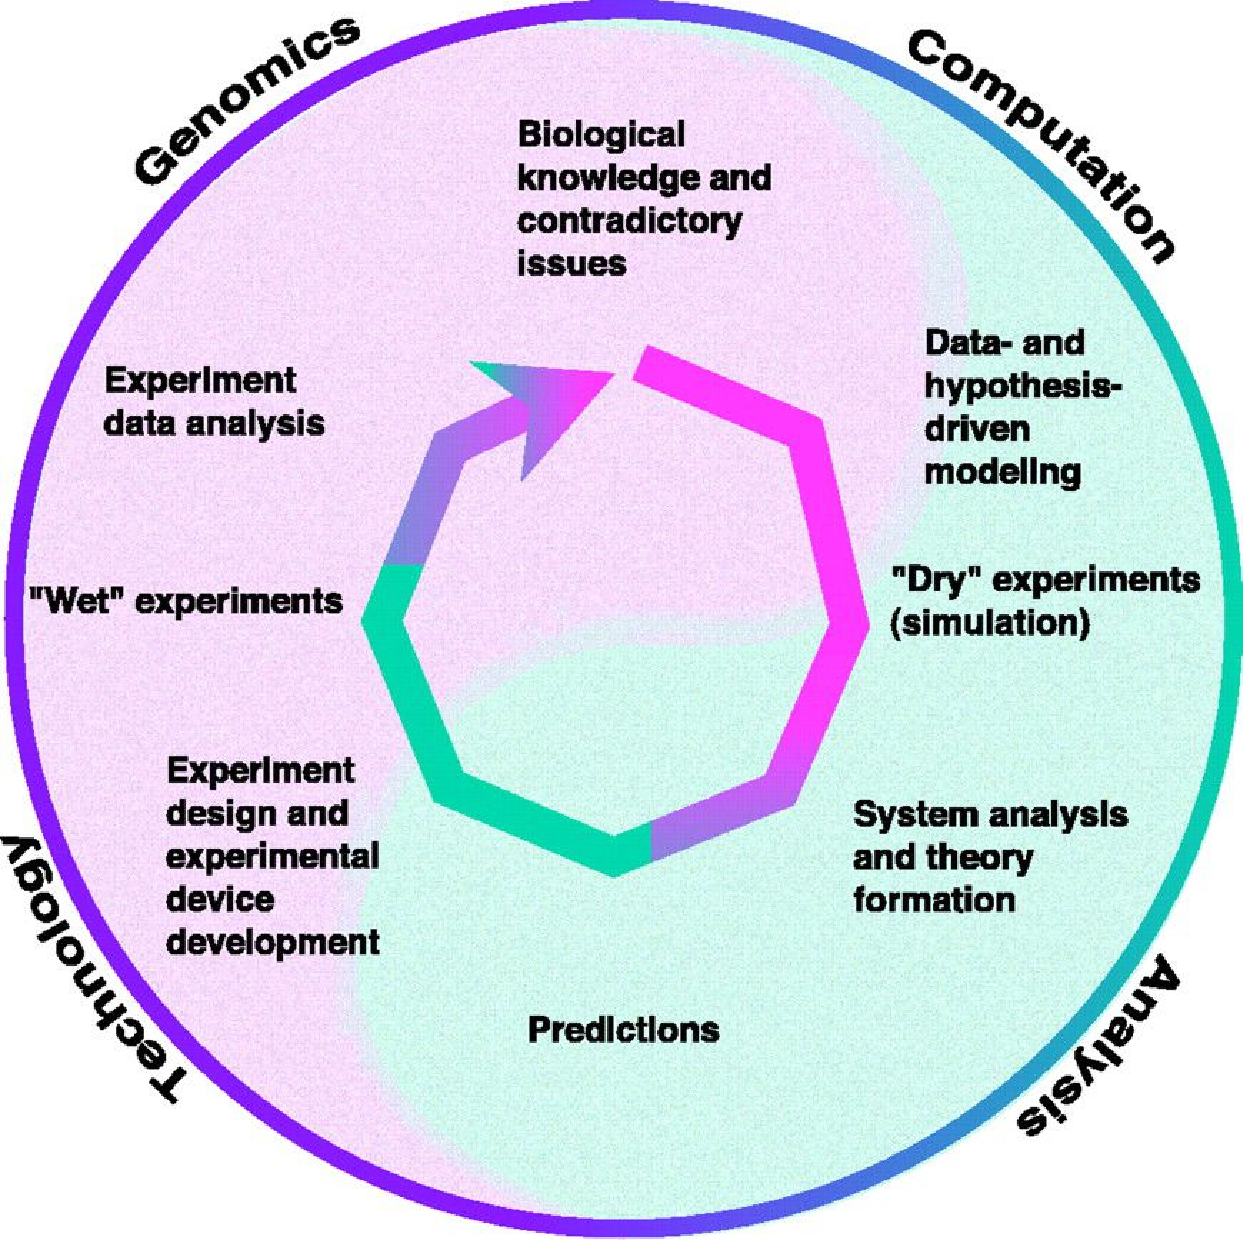
\includegraphics[width=0.6\textwidth]{Images/Other/systems biology.pdf}
    \caption{Combining Systems and Synthetic biology. Hypotheses of interest (e.g. the behaviour of a bacterial population after modifying a metabolic pathway) are used to create computational models. These are tested \textit{in silico}, or via 'dry' experiments, which can either support or deny the set of assumptions embedded in the model. When computer simulations reveal inadequacies in the hypotheses, these are adjusted with the information gleaned from the predicted behaviours. The revised models are then used to design new 'wet' experiments to perform, whose output is analysed and used to refine understanding of the issue. Figure from \cite{Kitano02systemsbiology:}. }
    \label{fig:syst_synth_bio}
\end{figure}

A complete understanding of biological systems can be harnessed to modify their normal course of action for beneficial applications. The field of synthetic biology, by combining technology, engineering and biological sciences, aims to alter existing cellular machinery for a variety of purposes. Bacteria, due to their unicellular nature and short regeneration time, are particularly suited for engineering complex metabolic pathways. Particularly, engineered microbes have been extensively used to produce therapeutic proteins, industrial enzymes, small molecular pharmaceuticals, chemicals, biofuels, and materials \cite{pmid23898328}. Together, systems and synthetic biology provide a new research framework that combines 'dry' (\textit{in silico} computer simulations) and 'wet' (carried out in the lab) experiments and data to iteratively propose and amend hypotheses (see Fig. \ref{fig:syst_synth_bio}). This novel approach promises to significantly speed up the development cycle, both for theoretical research questions and practical use cases, as well as reducing the costs involved in running expensive experiments. Therefore, it is crucial to develop faithful computational descriptions to yield insightful observations. 

Designing dry experiments requires mathematical models to describe the behaviour of the processes being investigated. Owing to our ability to observe and measure many diverse aspects of individual cells, much of the modelling in synthetic biology to date has focused on intracellular dynamics (e.g. variations in concentrations of proteins over time). As the reductionist school of thought became unable to explain the robustness and modularity shown by biological systems, the modelling paradigm began to shift to capture collective population-level features that extend beyond individual cells, thus becoming the perfect application for agent-based modelling.

\section{Agent-Based Modelling}\label{sec:theory_abm}
Agent-Based Modelling (ABM) is a computational modelling approach which captures emergent properties of dynamical systems by considering interactions between 'agents' and the environment. Agents can represent any entity of interest, such as a molecule, cell or multicellular organism, and each independently follows a prescribed set of rules. In a biological setting, these rules are often encoded as genetic circuits that drive cellular responses to particular stimuli. By simulating the behaviour of these virtual populations in realistic environments, it is possible to gain an understanding of how low-level cellular rules lead to the emergence of collective population-level behaviours \cite{pmid27903820}.

\begin{figure}[h]
    \centering
    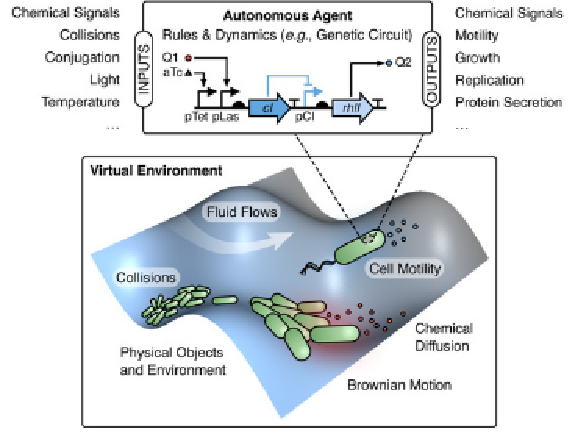
\includegraphics[width=0.7\textwidth]{Images/Other/abm.pdf}
    \caption{Agent-Based Modelling of cell populations. Agents' behaviour is determined by their internal state, the behaviour of other agents and the conditions of the surrounding environment. The system develops emergent properties as a result of the local interactions. The intracellular dynamics of each agent are specified by gene circuits with variable inputs such as chemical signals, collisions or temperature, and lead to different behaviours, e.g. replication, growth or protein secretion. The dynamics of gene circuitry is often specified as a system of ordinary differential equations (ODEs), specifying the rates of bio-chemical reactions. Figure from \cite{pmid27903820}. }
    \label{fig:abm}
\end{figure}

ABM offers two advantages over traditional modelling frameworks. Firstly, it captures minor differences that exist or can arise between agents, such as the varying levels of expression of a particular protein across a population due to intracellular noise. These differences are not trivial, as they can be leveraged to achieve novel functions. In \textit{Escherichia Coli} populations, for instance, cells can either be active or inactive depending on the concentration of stimulants, a property which improves the fitness of the population as a whole by ensuring that at least some cells can exploit changes in environmental conditions \cite{pmid14973486}. Other modelling approaches, by averaging out differences and assuming a uniform behaviour, fail to capture these features. The other major benefit of ABM is the ability to capture the multiplicity of interactions that agents can have. Direct physical interactions, where two agents meet, can be made more realistic by modifying them to be probabilistic, so that they do not always lead to the same behavioural responses. The environment itself can also act as a means for indirect interactions, such as as when pheromones are deposited to be sensed later by other individuals \cite{pmid26400200}. ABM easily incorporates this in the simulation, whereas traditional frameworks often struggle. A schematic overview of ABM can be seen in Figure \ref{fig:abm}.

Both agents and the environment can be specified via a collection of static properties (e.g. the cell walls' diffusivity rate or the dimensions of the space in which the agents are allowed to evolve) or dynamical ones. The latter are often in the form of systems of ordinary differential equations (ODEs), representing the rates of change for the concentration of chemical species. At each timestep in the simulation, the ODE model contained in each agent is run with input values determined by the state of the system. 

The model proposed in \cite{P21}, for instance, is a system of 12 ODEs representing cellular processes competing for three types of finite resources: \textit{cellular energy}, required to launch new biochemical processes, \textit{ribosomes}, necessary to translate mRNA, and \textit{proteome}, such that the expressing one type of protein reduces expression of others (Fig. \ref{fig:weisse_model}). The model relates gene expression with growth rate, and growth rate with a growing population of cells. For this reason, it is particularly suited to an agent-based exploration approach.

\begin{figure}
    \centering
    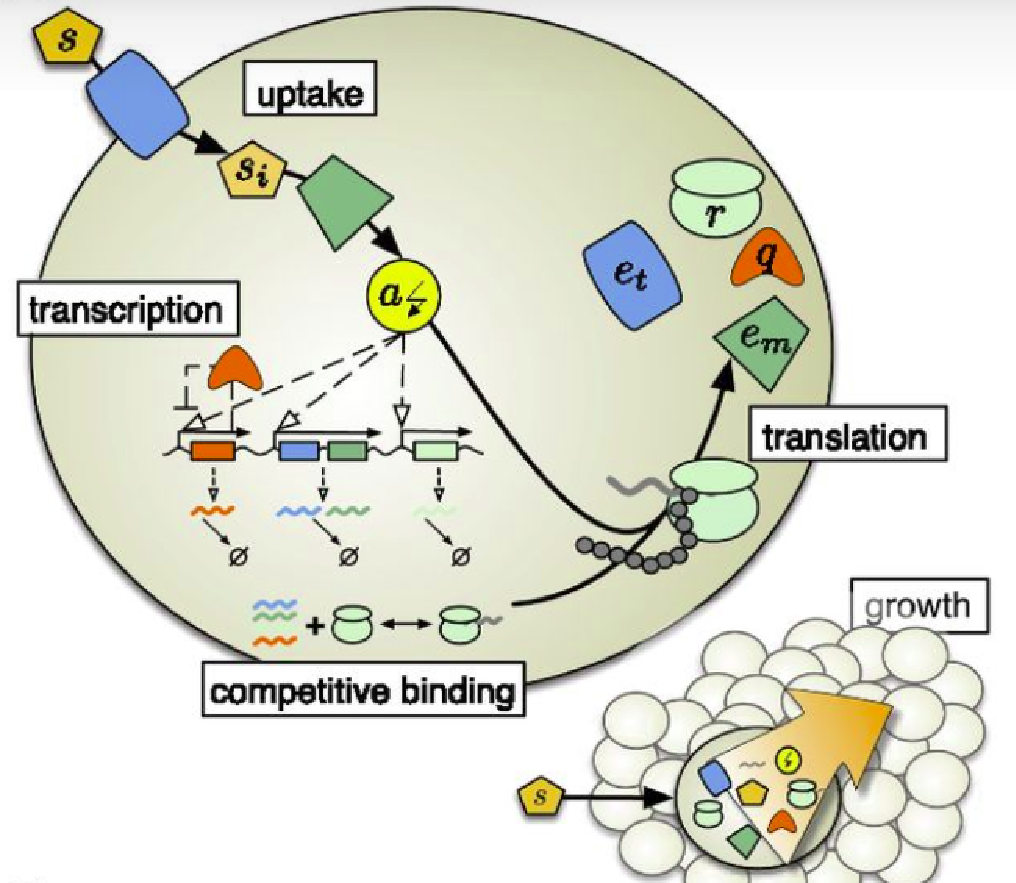
\includegraphics[width=0.6\textwidth]{Images/Other/weisse_model.pdf}
    \caption{Model presented in \cite{P21}. ODEs are used to describe the intake of an external nutrient, $s$, which, after being internalised as $s_{i}$, is used to produce cellular energy, $a$, which fuels a variety of cellular processes such as transcription and translation. The inset shows how every cell runs its own ODE system and together they all contribute to the growth of the population as a whole.}
    \label{fig:weisse_model}
\end{figure}

\section{Ordinary Differential Equations}\label{sec:odes}
The behaviour of agents in computational biology simulations is often described by a system of ordinary differential equations (ODEs). An ODE describes the rate of change of one or more dependent variables, $y$, as a function of a single independent variable, \textit{x}, more commonly referred to as \textit{t}, or time. In the context of computational and systems biology, ODEs are used the describe the concentrations of reactants used by chemical processes over time.

Most published models of biochemical reactions are non-linear and closed form solutions are not available. Accordingly, numerical integration methods have to be employed to study them \cite{Stadter2021}. These typically take the form of an \textit{initial value problem}, where the value of $y$ is provided at \textit{$t_{0}$}. The final solution is obtained iteratively over a specified number of timesteps, by applying the numerical method at time \textit{$t_{i}$} to the result of the integration at \textit{$t_{i-1}$}.

The timescales for the reaction rate of the molecular processes can differ by orders of magnitude \cite{pmid24098642}, a phenomenon captured by so-called \textit{stiff} ODEs. Stiffness occurs whenever there are slowly changing solutions combined with rapidly changing components. An example of a non-stiff and stiff ODE is shown in Figure \ref{fig:vanderpol} and Figure \ref{fig:vanderpol_stiff}, respectively, illustrating the exact solutions for the van der Pol equation, defined as 

\begin{equation}\label{eq:vanderpol}
\begin{array}{lcl} y_{1}' &  = & y_{2}, \\ y_{2}' & = & \mu(1-y_{1}^{2})y_{2}-y_{1}. \end{array}
\end{equation}

where $y'$ refers to the first derivative of $y$.

\begin{figure}[h]
    \centering
        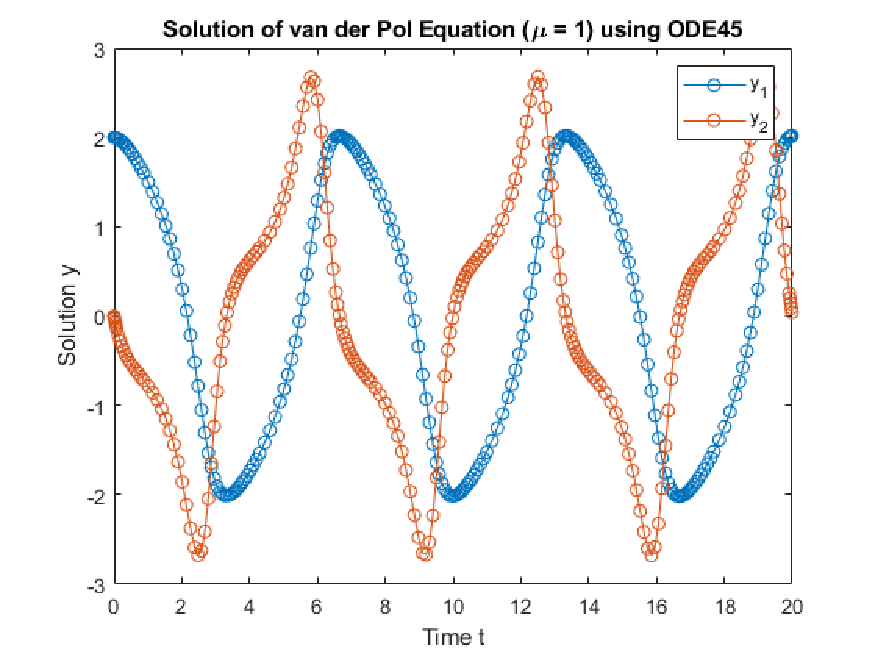
\includegraphics[width=0.5\textwidth]{Images/Other/vanderpol.pdf}
    \caption{van der Pol equation with $\mu=1$, solved with MATLAB's ode45 function \cite{ode45}. Note how $y_{1}$ and $y_{2}$ change over the same timescale.}
    \label{fig:vanderpol}
\end{figure}

\begin{figure}[h]
    \centering
        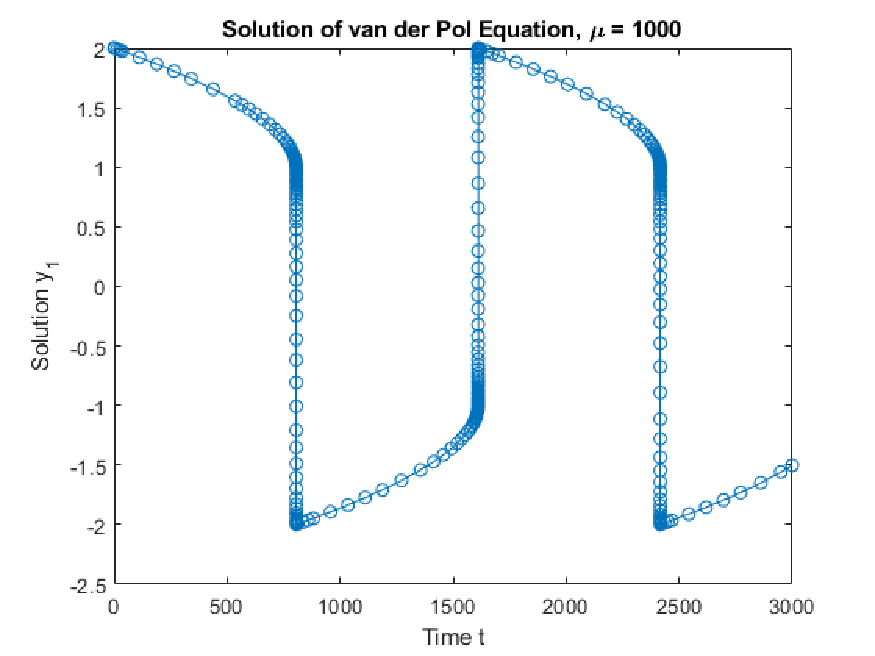
\includegraphics[width=0.5\textwidth]{Images/Other/vanderpol_stiff.pdf}
    \caption{van der Pol equation with $\mu=1000$, solved with MATLAB's ode15s function \cite{ode15s}. The same equation becomes stiff when changing the value of $\mu$. Note how the behaviour of $y_{1}$ changes compared to its stiff counterpart with $\mu=1$ in Fig. \ref{fig:vanderpol}. $y_{2}$ is not plotted for scaling reasons.}
    \label{fig:vanderpol_stiff}
\end{figure}

The step size taken by an ODE solver is forced down to an unreasonably small level in comparison to the interval of integration when dealing with stiff systems. The step size can be so small that traversing a short time interval might require millions of evaluations, if not leading to a failure of the integration altogether. Fortunately, stiff ODE solvers that take this problem into account do exist and have been extensively benchmarked \cite{Stadter2021}. The choice of an appropriate ODE solving routine is particularly important when the ODE system has to be simulated and solved a significant number of times, such as in the context of parameter inference.





\section{Parameter Inference}\label{sec:param_inference}
The systems of ODEs used to describe the dynamics of biological processes introduce various unknown parameters that need to be estimated efficiently from a set of experimental observations. One of the major challenges faced by parameter inference in the context of computational systems biology is the limited size of the set of available observations, given the complexity of the models and the time and resources needed to run them. This problem is compounded by the fact that some species evolve over timescales orders of magnitude apart, a property represented by stiff ODEs. Furthermore, the data available frequently contains noise, caused by either the instruments used to capture it (e.g. the microscope's measurement error), or simply by the stochasticity of the processes themselves.

Formally, we are given a system of ODEs representing the biochemical processes as follows

\begin{equation}
    \frac{d\textbf{x}}{dt} = \textit{\textbf{f}}(\textbf{x}, t, \textbf{p}),
\end{equation}

where the state vector $\textbf{x} = (x_{1}, x_{2}, ..., x_{N})$ represents the concentrations of $N$ species and $\textbf{p} = (p_{1}, p_{2}, ..., p_{K})$ are $K$ parameters of the model \cite{pmid33206658}. We are also given the set of initial observations at time $T_{0}$

\begin{equation}
    \textbf{x}(T_{0}) = \textbf{x}_{0},
\end{equation}

which is used to make an initial random guess as to what the values of the parameters $\textbf{p}$ could be. From here, by repeatedly running the model and collecting observations, the parameter inference procedure refines its estimate of the values of the variables. This is represented as follows

\begin{equation}
    \textbf{y} = \textit{\textbf{h}}(x) + \epsilon(t), \quad \epsilon(t) \sim \mathcal{N}(\mu,\,\sigma^{2}),
\end{equation}

where $\textbf{y}$ are experimental observations consistent with the ODE system, which possibly contains noise $\epsilon$ of Gaussian type with mean $\mu$ and standard deviation $\sigma$. The output function \textit{\textbf{h}} is defined as part of the experiment design, however it is often of the form

\begin{equation}
    \begin{bmatrix}
        y_{1} \\
        y_{2} \\
        ... \\
        y_{N} \\
    \end{bmatrix}
        =
    \begin{bmatrix}
        x_{1} \\
        x_{2} \\
        ... \\
        x_{N} \\
    \end{bmatrix}
    +
    \begin{bmatrix}
        \epsilon_{1} \\
        \epsilon_{2} \\
        ... \\
        \epsilon_{N} \\
    \end{bmatrix}.
\end{equation}

Assuming there is a set of parameters $\textbf{p*}$ such that $\textit{\textbf{f}}(\textbf{x}, t, \textbf{p*})$ is a sufficiently accurate mathematical description approximating reality, i.e. all the relevant knowledge about the biological processes is incorporated correctly into the vector function $\textbf{\textit{f}}$, we define a vector of discrepancies between the model values $\textit{\textbf{p*}}$ and the experimental values $\bm{\hat{p}}$ as

\begin{equation}
    \textbf{e}(\bm{\hat{p}}) = |\textit{\textbf{f}}(\textbf{x}, t, \textbf{p*}) - \textit{\textbf{f}}(\textbf{x}, t, \bm{\hat{p}})|.
\end{equation}

The task of parameter inference can then be expressed as finding the set of parameters $\textit{\textbf{p}}$ that minimizes $\mathbf{e}(\textit{\textbf{p}})$, often referred to as the \textit{objective} function, 

\begin{equation}
    \textit{\textbf{p}} = \operatorname*{arg\,min}_\p \textit{\textbf{p}} \textbf{e}(\textit{\textbf{p}} ).
\end{equation}

The task of minimising the objective function is called \textit{optimization}, and although a variety of approaches exist to perform it, these can broadly be classified into two categories: \textit{local} and \textit{global} optimization methods.

A parameter vector $\bf{\hat{p}}$ is said to be a local minimizer of $\textbf{e}$ if it gives the lowest obtainable objective function value in the neighbourhood of a starting point

\begin{equation}
    \mathbf{\hat{p}}_{local} = \operatorname*{arg\,min}_\p \textit{\textbf{p}} \textbf{e}(\textit{\textbf{p}})  \quad \forall || \textit{\textbf{p}} - \mathbf{\hat{p}}_{start} || < \delta, \quad \delta > 0.
\end{equation}

A global optimizer, on the other hand, gives the lowest obtainable objective function value from an arbitrary starting point:

% Horizontal space smaller than \quad %
\newcommand{\Hquad}{\hspace{0.4em}} 

\begin{equation}
    \mathbf{\hat{p}}_{global} = \operatorname*{arg\,min}_\p \textit{\textbf{p}} \textbf{e}(\textit{\textbf{p}})  \quad \forall \mathbf{p} \Hquad \text{in the parameter space}.
\end{equation}

Local optimizers work by computing the gradient of the objective function with respect to the parameter vector. The gradient $\nabla$ is simply a vector containing the partial derivative of the function with respect to each $\textit{p}_{i}$ in $\textit{\textbf{p}}$

\begin{equation}
    \nabla \textbf{e}(\mathbf{\hat{p}}) = 
    \begin{bmatrix}
      \frac{\partial \textbf{e}}{\partial \textbf{p}} (\mathbf{\hat{p}})  
    \end{bmatrix}.
\end{equation}

At its minimum, the gradient of the objective function with respect to the parameters vanishes, i.e. is equal to zero. Local optimization methods employ this fact to explore the parameter space by following the opposite direction of the steepest gradient, which is proven to converge to a local minimum \cite{Curry1944TheMO}. 

Multiple issues arise when adopting local optimization in the context of systems biology. Firstly, the objectives to optimize are often 'black-box' functions, meaning that no assumptions about their shape can be made, including the computability of their gradient. This is even more emphasised in agent-based simulations by the stochastic nature of the interactions and evolution of individual agents and the entire population. Secondly, assuming that the gradients can be computed, the non-linearity of biological systems can lead to multimodal landscapes (more than one minimum are present) \cite{article}. Local methods tend to get trapped in local minima and, although a number of high-performing software packages are available (Copasi \cite{hoops2006copasi}, PottersWheel \cite{maiwald2008dynamical}), these often require multi-start strategies (repeatedly applying the local method starting from a number of different initial vectors) to address the presence of multiple minima \cite{10.3389/fams.2019.00055}. When we consider the additional burden of numerically solving the system of ODEs for every simulation iteration, local optimization methods often become not viable due to their high computational costs. It is therefore desirable to minimise the number of stochastic simulations required to perform parametric inference for noisy biological systems \cite{https://doi.org/10.48550/arxiv.1403.8057}.

Global optimization methods are designed to address the issues described above. They do not require knowledge of the gradients, only an order relation of the form $\textbf{e}(\textbf{p}_{1}) < \textbf{e}(\textbf{p}_{2})$ for the points in the parameter space \cite{pmid19215296}. Certain global optimizers are stochastic in nature, meaning that although the theoretical global minimum cannot not be reached, solutions in its vicinity can be located with relative efficiency. In practice, the solutions are satisfactory enough and can be achieved in modest computation times. Finally, global optimization methods do not required any transformation of the original problem, which can be thus treated as a black box \cite{pmid14559783}. This work focuses on Bayesian inference, a particular type of stochastic global optimization.

\subsection{Bayesian Inference}\label{sec:bayesian_inference}
Bayesian methods are a family of statistical modelling approaches used, among other applications, for parameter inference. They are particularly suited to the context of systems biology \cite{P33} due to the problem of parameter \textit{identifiability}. Because of the high-dimensionality of the parameter space and the limited, noisy amounts of data available from expensive biological experiments, multiple sets of parameters equivalently describe the experimental data. When parameters are non-identifiable, a single parameter set is insufficient to describe the feasible space of parameters associated with the model \cite{8374537}.

Bayesian methods solve this problem by modelling the entire probability distribution of the unknown parameters, rather than just a point-estimate, given the experimental data. This allows both determination of best-fit parameters, as well as allowing the modeller to incorporate and prior information they might have about the parameters \cite{pmid24457334}.

Bayesian inference estimates a set of parameters $\theta$ by merging the available (prior) information about the model with the information obtained by observing new data $\mathscr{D}$. This is represented by Bayes’ theorem \cite{P34}:

\begin{equation}
    \pi(\theta | \mathscr{D}) = \frac{\mathbb{P}(\mathscr{D} | \theta)\pi(\theta)}{\mathbb{P}(\mathscr{D})}.
\end{equation}

Where the \textit{prior} $\pi(\theta)$ and the \textit{posterior} $\pi(\theta|\mathscr{D})$ summarise the available information about $\theta$ before and after considering the data $\mathscr{D}$, respectively. The other two terms are $P(\mathscr{D})$, the \textit{marginal probability} of observing $\mathscr{D}$, and $P(\mathscr{D}|\theta)$, the \textit{likelihood}. The former is a normalization constant, whereas the latter represents the probability of observing the data $\mathscr{D}$ given the current parameterization.

One commonly adopted instance of Bayesian methods in the field of systems biology is Markov Chain Monte Carlo. Example applications include parameter inference for influenza transmission \cite{mathews2007biological} or finite resource allocation in molecular processes \cite{P21}, illustrated in Section \ref{sec:theory_abm}. 


\subsection{Markov Chain Monte Carlo}\label{sec:mcmc_theory}
Markov Chain Monte Carlo (MCMC) is a sampling technique that generates a chain of parameters $\theta^{1}, \theta^{2}, ..., \theta^{d_{s}}$ by exploring the posterior distribution $\pi(\theta | \mathscr{D})$ \cite{P44}. 
The samples are generated form a Markov chain that serves as an approximation of the distribution of interest, or \textit{target}. It can be proven that given enough sampling the stationary distribution of the chain (a distribution $\pi$ that does not change as more samples are obtained, i.e. $\pi = \pi\textbf{P}$ for a given transition matrix $\textbf{P}$) is the target \cite{P45}.

Each iteration of an MCMC algorithm follows two steps. Firstly, a point $\theta^{k}$ in the parameter space is proposed by sampling it from a proposal distribution

\begin{equation}
    \theta^{k} \sim \mathbb{Q}(\theta^{k}, \theta^{k-1}).
\end{equation}



The proposal density $\mathbb{Q}(\theta^{k}, \theta^{k-1})$ depends on the previous chain member, $\theta^{k-1}$, and might be any distribution from which we can sample, such as a Gaussian centered at $\theta^{k-1}$.


In the second step, the proposal is either accepted or rejected based on whether the value of the posterior evaluated at the proposal is higher than its evaluation at the previous proposal. The rule is represented by the following

\begin{equation}
    p_{a} = min\left\{{1, \frac{P(\mathscr{D} | \theta^{k})}{P(\mathscr{D} | \theta^{k-1})} \frac{\pi(\theta^{k})}{\pi(\theta^{k-1})}} \frac{\mathbb{Q}(\theta^{k-1},\theta^{k})}{\mathbb{Q}(\theta^{k},\theta^{k-1})} \right\}.
\end{equation}



If the proposal is accepted, it is used as the reference point for the next iteration of the algorithm, otherwise it is discarded.


As already mentioned, the stationary distribution of the chain is the target, however it is not straightforward to determine the convergence of the chain at any instant \textit{t} in time \cite{oro22547}. This is because the convergence is not to a point, but to a distribution of a sequence of generated values to another distribution. No single diagnostic tool exists to assess convergence, and several methods are used together to approximate convergence measurement \cite{doi:10.1198/1061860031347}. However, the number of iterations recommended to be reasonably confident that MCMC has converged is highly computationally demanding, and not viable for commercial hardware \cite{P37}. This limitation is even more restricting when obtaining each sample is expensive, which, as already mentioned,  is the case for complex ODE systems in computational biology.

Another consideration to be made on MCMC regards the choice of the proposal distribution. Because of the dependence of each sample on the previous one, the choice of an appropriate proposal distribution becomes crucial to minimise the correlation between samples which could lead to slower convergence or even becoming trapped in local optima during the search for global ones \cite{rosenthal2011optimal}. The hyperparameters of the proposal are often manually tuned by field experts and in general what works for one domain cannot be extended to others. A solution to the problem would be to employ an approach that is inherently designed to minimise the amount of sampling required and does not require exhaustive tuning of a proposal function. Bayesian Optimization is designed to achieve this goal.






\subsection{Bayesian Optimization}\label{sec:BO_theory}


Bayesian Optimization (BayesOpt) is a class of algorithms aimed at optimizing objective functions that are very costly (in terms of time, money or other resources) to evaluate \cite{Jones1998EfficientGO}.

BayesOpt algorithms try to minimise the number of evaluations of the objective by employing an acquisition function which identifies the next point to sample in order to maximize the informational gain of the sampling  procedure by balancing the “exploration-exploitation” trade-off (sample points that are far from the current sample to learn about the function in an unobserved area vs. pick the next sample near the current one when this is believed to be near an optimum).

BayesOpt consists of two main components:
\begin{itemize}
    \item A Bayesian statistical model for modelling the objective function, a “surrogate” of it. The goal of the surrogate is to provide a posterior probability distribution that describes potential values for the objective function at a specific candidate point (Fig.\ref{fig:GP}, Top panel).
    \item An acquisition function for deciding where to sample next. It measures the value that would be generated by evaluation of the objective function at a new point, based on the current posterior distribution over the target (Fig.\ref{fig:GP}, Bottom panel).
\end{itemize}

BayesOpt is often used in conjunction with other parameter estimation methods. For instance, it is used in adaptive MCMC to tune the hyperparameters of the Markov Chain \cite{mahendran2012adaptive}. However, to the best of my knowledge, it has not been applied in isolation for the purpose of parameter inference in the field of Systems and Computational biology.

BayesOpt can solve many of the problems encountered by traditional MCMC since it is, by design, a 'black-box, derivative-free global optimizer' \cite{Jones1998EfficientGO}:

\begin{itemize}
    \item Black-box, since no special structure about the function, like convexity or linearity, is known and can therefore be exploited;
    
    \item Derivative-free, since no first- or second-order derivatives are required, only the objective itself;
    
    \item Global, meaning it globally samples over the objective, rather than locally like in based on Markov Chains-based methods.
\end{itemize}

\begin{figure}[ht]
    \centering
    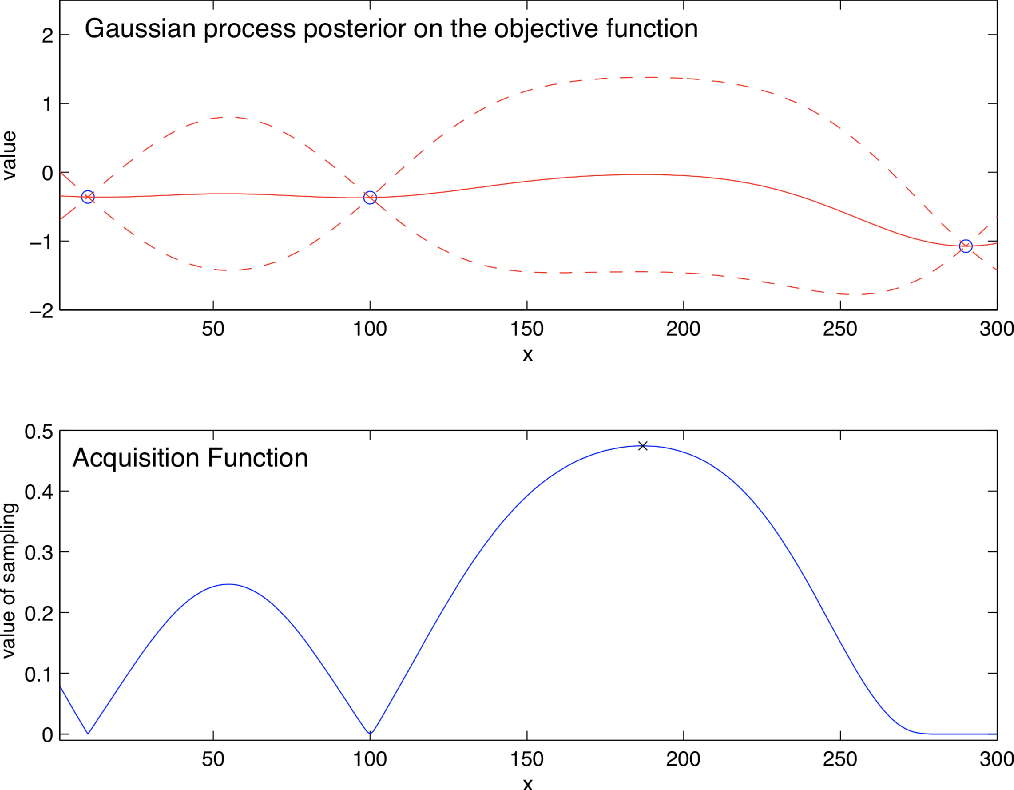
\includegraphics[width=.6\linewidth]{Images/Other/bayesOpt.png}
    \caption{\textit{Top panel}: The surrogate model, in this case a Gaussian Process, used to approximate the target. The blue dots represent observations of the objective function. The solid line is the estimate of the target. The dashed lines are Bayesian credible intervals, representing the confidence on the range of possible values that the target evaluates to at a specific point.
    \textit{Bottom panel}: The acquisition function, whose maximum indicated by the 'x' represents the next point to sample on the surrogate. The acquisition function balances exploration (leading to sample in areas with bigger confidence intervals, representing uncertainty in that area) and exploitation (leading to sample in areas where an optimum is thought to be present based on previous samples).}
    \label{fig:GP}
\end{figure}


\chapter{Implementation \& Experiments}\label{ch:experiments}

This chapter presents the software libraries, algorithms and implementation decisions adopted in the comparative analysis of Bayesian Optimization and Markov Chain Monte Carlo techniques for parameter inference. It discusses alternative tools and approaches for individual components of the experimental setup: Agent-Based Modelling (Section \ref{sec:abm}), BayesOpt (Section \ref{sec:BO}) and MCMC (Section \ref{sec:mcmc}). Finally, it outlines the experimental conditions under which the two methods have been explored (Section \ref{sec:experiments}).

\section{Agent-based Cell Simulators}\label{sec:abm}
The first step to build an agent-based simulation is to find the correct software that meets our modelling criteria. Sections \ref{sec:gro} - \ref{sec:bsim} illustrate the advantages and limitations of different biological modelling packages. Although the perfect tool does not exist, we would like our candidates to strike a good balance between complexity of the simulation and ease of deployment. The properties to look for are:

\begin{itemize}
    \item Customisability of growth rate and division rules;
    \item Stochasticity in agent-agent and agent-environment interactions;
    \item Support for stiff ODE solving.
\end{itemize}

Table \ref{tab:abm_tools} shows an overview of the packages I have tested and their properties.

\begin{table}
    \centering
    \begin{tabular}{clcccc}
    \toprule[1pt]
        & & & & & \\
        & & Gro & CellModeller & CompuCell 3D & Bsim \\ \cline{3-6}
        
        \multirow{10}{0.15\textwidth}{\textbf{Agent dynamics and features}}
        & Simple rules & \checkmark & \checkmark & \checkmark & \checkmark \\ 
        & Advanced rules & \checkmark  & \checkmark & \checkmark & \checkmark \\ 
        & ODEs & & \checkmark & \checkmark & \checkmark \\
        & DDEs & & & & \checkmark \\
        & Chemical equations & & & & \\
        & Stochastic dynamics & \checkmark & \checkmark & \checkmark & \checkmark \\ 
        & Motility & \checkmark & & \checkmark & \checkmark \\
        & Chemotaxis & \checkmark & & \checkmark & \checkmark \\
        & Cell replication & \checkmark & \checkmark & \checkmark & \checkmark \\ \
        & Cell morphology & \checkmark & \checkmark & \checkmark & \\[3.5mm] \cline{1-6}
        & & & & & \\
        
        \multirow{4}{0.15\textwidth}{\textbf{Environment}}
        & 2D & \checkmark & & \checkmark & \\
        & 3D & & \checkmark & \checkmark & \checkmark \\
        & Chemical diffusion & \checkmark & \checkmark & \checkmark & \checkmark \\
        & Complex objects & & & \checkmark & \checkmark \\ [3.5mm] \cline{1-6}
        & & & & & \\
        
        & Language & C++ & Python & C++/Python & Java \\
        & Reference(s) & \cite{Jang2012} & \cite{pmid23651288} & \cite{pmid22482955} & \cite{pmid28585809} \\
        & & & & & \\
        
    \bottomrule[1pt]
    \end{tabular}

    \caption{Overview of the Agent-Based Modelling tools tested and their properties. Table adapted from \cite{pmid27903820}. \\ \\
    \textbf{Description of properties}  \vspace{0.5em} \\
    \textbf{Simple Rules}: a limited subset of commands are available to control agent behaviours; \\ 
    \textbf{Advanced Rules}: access to a full programming language is provided to control agents; \\
    \textbf{ODEs}: agents can use ordinary differential equations to describe their internal state;\
    \textbf{DDEs}: agents can use delay differential equations to describe their internal state; \\
    \textbf{Chemical equations}: cellular chemical reaction networks can be simulated; \\
    \textbf{Stochastic dynamics}: the internal state of an agent and the interactions with other agents can be stochastic, i.e. upon meeting another agent, there is a probability that they interact;\\
    \textbf{Motility}: agents can move freely within the environment and functionality to manage collisions/interactions is available; \\
    \textbf{Chemotaxis}: a realistic implementation of chemotaxis, i.e. chemically induced motility, is available to control cellular movement; \\
    \textbf{Cell replication}:  agents are able to replicate over time; \\
    \textbf{Cell morphology}: agents can take an arbitrary shape or have the option to take one of multiple predefined shapes;\\
    \textbf{2D}: visualizations in 2D of the simulations are available;\\
    \textbf{3D}: visualizations in 3D of the simulations are available;\\
    \textbf{Chemical diffusion}: movements of chemical species in the environment can be customised; \\
    \textbf{Complex objects}: augment behaviour and properties of individual agents by extending desired classes.
    }\label{tab:abm_tools}
\end{table}

\subsection{Gro}\label{sec:gro}
Gro \cite{Jang2012}, developed at the University of Washington, was the first candidate ABM tool I adopted. This choice was driven by the simplicity of gro which provides a friendly user interface to the underlying C++ source code, while allowing for detailed model descriptions. After its first release in 2013, gro significantly surpassed the complexity of the biological modelling tools available at the time. It introduced, for instance, customisable morphology for growing microcolonies of bacteria and design of gene circuit interactions. 

A simple example showcasing the simplicity of gro is shown below, where production, dilution and degradation of the gfp protein produced by \textit{E. coli} are simulated.

\begin{lstlisting}[basicstyle=\small]
program make_gfp ( k1, k2, m ) := {

  // initialize gfp copy number
  gfp := m;

  // produce gfp
  rate ( k1 ) : { gfp := gfp + 1 }

  // degrade gfp
  rate ( k2 * gfp ) : { gfp := gfp - 1 }

};

// compute production rate needed for 100 copies of gfp per cell
alpha := - log ( 0.5 ) / 20.0; // dilution rate
k1 := 100 * alpha;             // production rate

// make a new cell
ecoli ( [ x := 0, y := 0 ], program make_gfp ( k1, 0.001, 0 ) );
\end{lstlisting}

As part of the inspection for the suitability of gro, I learned its specification language. The overall logic and syntax are easily provided within a programming background, however I used the opportunity to familiarise myself with fundamental biological concepts and how these are implemented in code. This proved to be an important stepping stone towards more complex tools and simulations explored in later stages. \\ \newline
Eventually, I discarded gro as the ABM tool of choice for two reasons. Firstly, it can only run on Windows or Mac operating systems, thus being incompatible with Linux, the os powering the machine on which the experiments that have been run. I attempted to overcome this obstacle by setting up a Windows Virtual Machine, however the virtualization software proved to be a considerable speed bottleneck. As Bayesian Optimization requires multiple simulation iterations to be run, such a slowdown was not viable.
Secondly, gro does not offer the possibility of specifying agents' internal state via a system of ordinary differential equations (ODEs). This limitation is quite restrictive in this work's context, as a thorough parameter inference analysis would treat variables exhibiting more complex behaviours.

\subsection{CompuCell3D}\label{sec:compucell3d}
CompuCell3D (CC3D) \cite{pmid22482955}, originally developed at the University of Indiana in 2012, is a powerful ABM tool that allows rapid construction of multi-scale simulations for a variety of biological domains, including bacterial populations. Compared to gro, CC3D offers extensive \href{https://compucell3d.org/Manuals}{instruction manuals}, \href{https://compucell3d.org/DeveloperZone}{installation guides} and \href{https://www.reddit.com/r/CompuCell3D/}{support forums}. More crucially for the purpose of this work, it supports ODE-specified agent behaviour. It is actively maintained and utilized in different research areas as of the time of writing.

I decided to experiment with CC3D for multiple reasons:

\begin{enumerate}
    \item Rich graphical user interface  which allows for quick customizability of the simulations, as well as providing detailed representations for qualitative visual analysis. An example of CC3D's GUI can be seen in Fig. \ref{fig:CC3D};
    \item Source code for simulation directly written in Python, which brings two benefits. Firstly, since Python is the language I am most familiar with, it held promise of speeding up the development process. Secondly, it would be easier to interface with BayesOpt libraries also written in Python;
    \item Runs on Linux, thus avoiding the need for a virtual machine and associated computational bottleneck;
    \item Supports Systems Biology Markup Language (SBML) \cite{pmid31219795}. Many systems biological models are disseminated in SBML, a widely adopted protocol in the computational biology field. Importing a SBML file directly rather than having to manually write code for the simulation significantly reduces development time.
\end{enumerate}

\begin{figure}
    \centering
    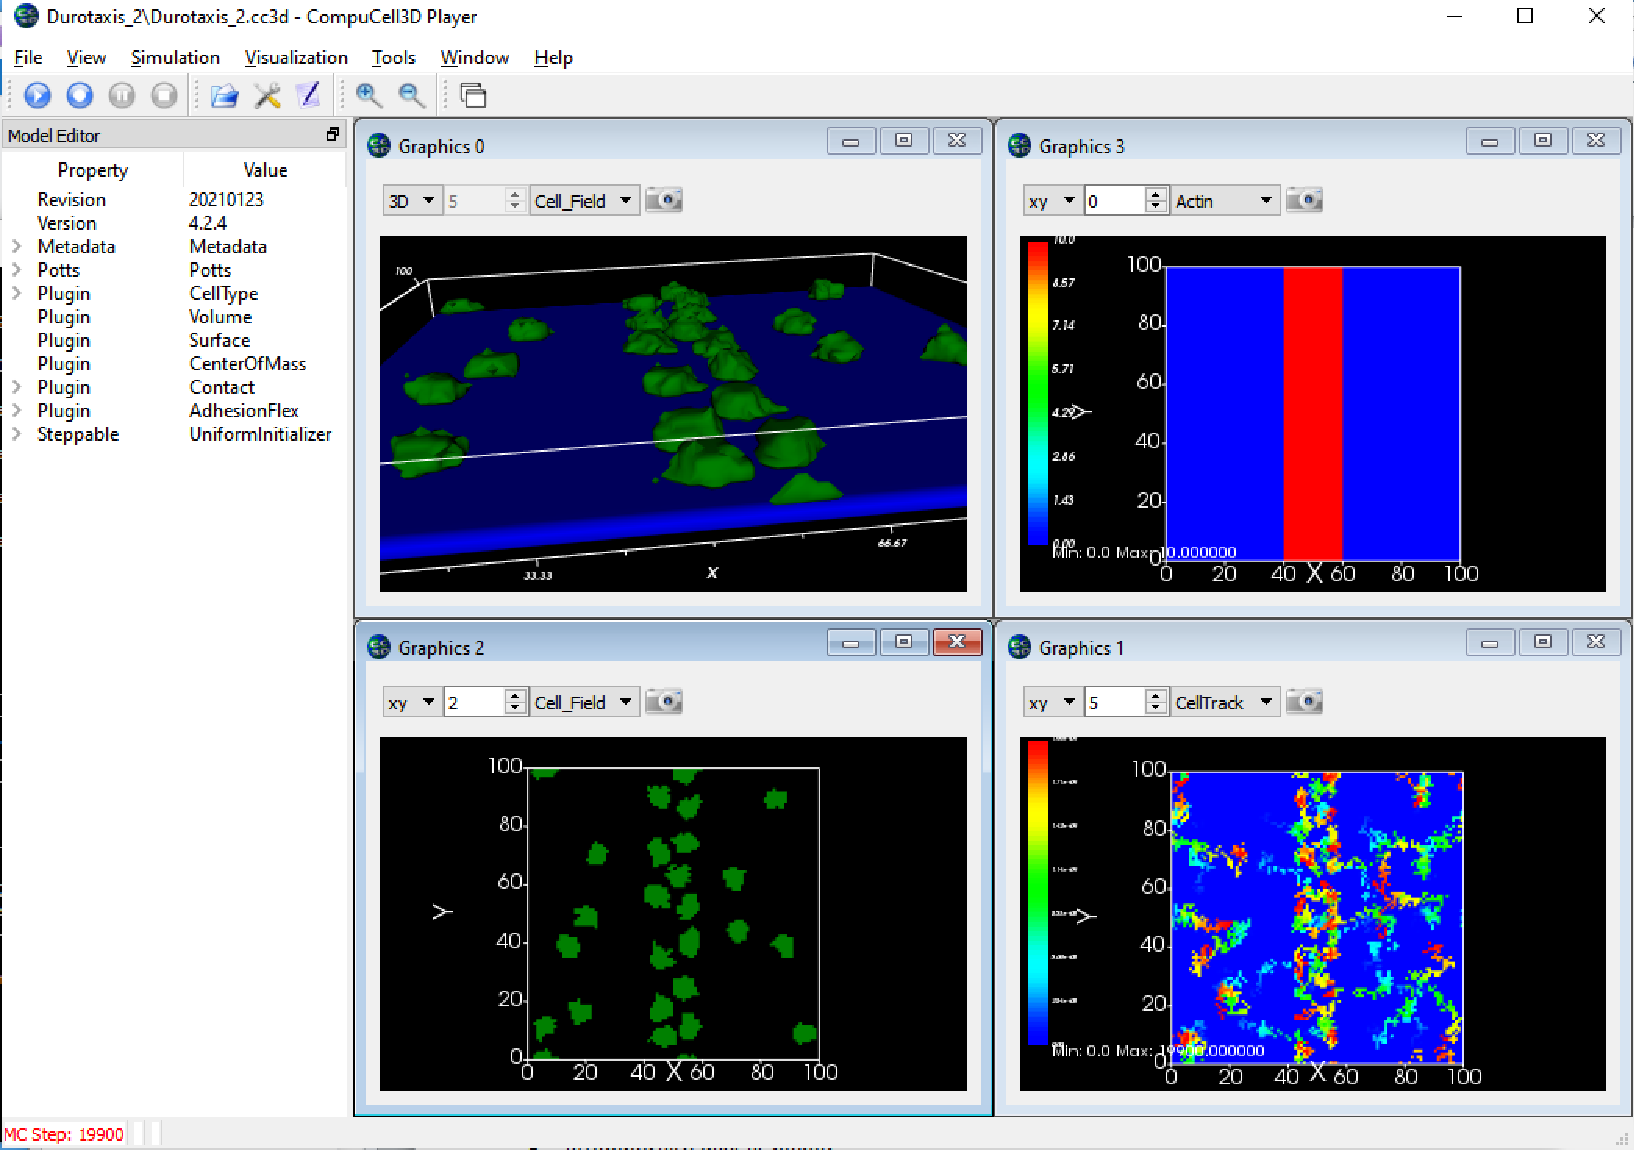
\includegraphics[width=0.8\textwidth]{Images/Other/CC3D.pdf}
    \caption{CC3D's GUI offers quick shortcuts to customize running simulations, as well as rich representations for qualitative visual analysis.}
    \label{fig:CC3D}
\end{figure}

Although yielding some promising initial results, I encountered difficulties in installing and linking the external modules for ODE support (\href{https://tellurium.analogmachine.org/}{Tellerium}, \href{http://libroadrunner.org/}{libRoadRunner}). After extensive research and reaching out to some of the CompuCell3D developers, I was not able to solve the problem. As the process was taking significantly long, I eventually decided to explore further alternatives.




\subsection{CellModeller}\label{sec:cellmodeller}
CellModeller \cite{pmid23651288}, developed at the University of Cambridge, is a Python-based ABM framework offering customisable intra- and extracellular dynamics with ODE support. Although not maintained anymore, the concise tutorials allow to quickly deploy complex simulations. I have adopted CellModeller in the early stages of BayesOpt experimentation by making use of existing examples (specifically the circuit described in Fig. \ref{fig:cellmodeller}) that contain ODE-defined behaviour. This allowed me to create a successful proof-of-concept without the burden of implementing the simulation itself. 

\begin{figure}
    \centering
    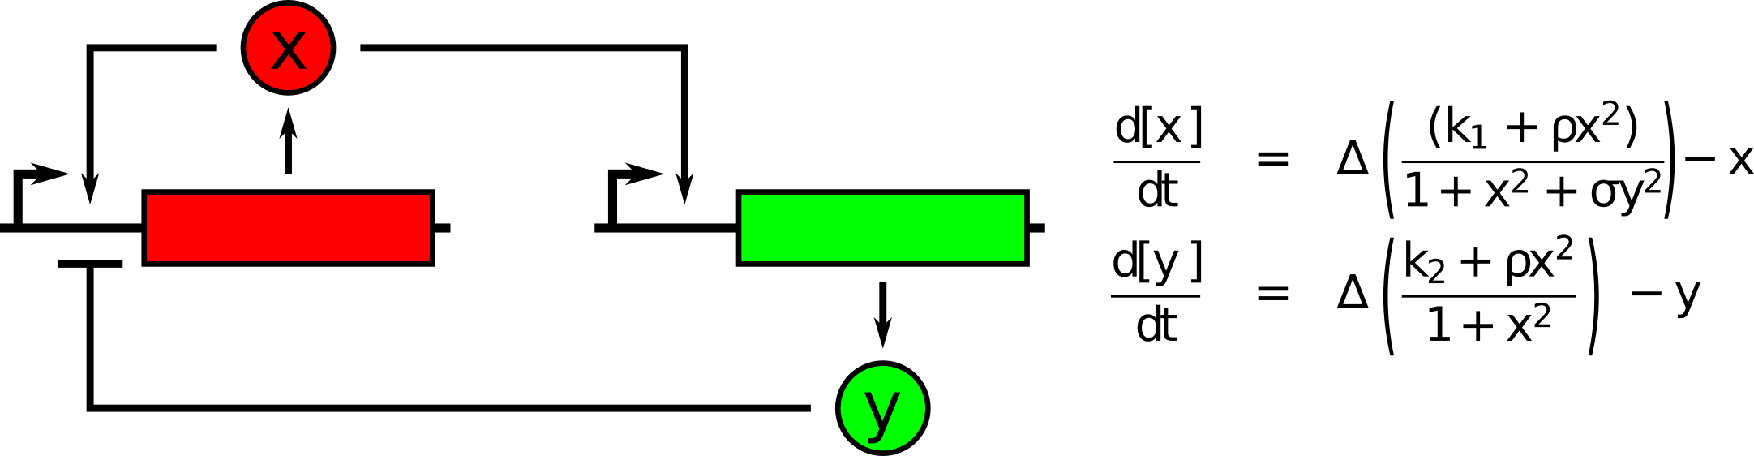
\includegraphics[width=0.7\textwidth]{Images/Other/CellModeller_tutorial2b_circuit.pdf}
    \caption{Simple gene circuit in which two species, $x$ and $y$, are produced at the rates specified by the corresponding equations. Out of the four variables $k_{1}$, $k_{2}$, $\rho$ and $\sigma$, only one, $\rho$, was inferred via BayesOpt as part of a proof-of-concept.}
    \label{fig:cellmodeller}
\end{figure}

The major limitation of CellModeller is that it does not support stiff ODE solvers. As mentioned in Section \ref{sec:odes}, these are often present in systems biology, as parameters vary over different orders of magnitude. I therefore decided to discard CellModeller as the final ABM tool of choice, while looking for alternatives that would support more complex simulations with stiff ODEs.

\subsection{Bsim}\label{sec:bsim}
Bsim \cite{pmid22936991, pmid28585809} is a biological ABM tool that overcomes the limitations posed by the alternatives discussed above. Written in Java, it follows an object-oriented paradigm that requires knowledge of software engineering fundamentals, thus making not ideal for practitioners outside the computing field. It contains a variety of reusable, isolated components representing common bacterial traits applicable to numerous kinds of models, thus saving time and effort in the development process; it supports complex intracellular dynamics and stiff ODEs; it allows customisability of agents' morphology, division rules and growth rate, as well as environmental properties and interactions; finally, it offers an attractive GUI for 3D visualizations. For these reasons, I considered it the best ABM package candidate and I adopted it throughout the BayesOpt experiments.

\section{Bayesian Optimization}\label{sec:BO}
The package I have chosen to perform Bayesian Optimization is GPyOpt \cite{GPyOpt, GPyOpt_home}. It is one of the first libraries for Bayesian Optimization written in Python. Despite its age and end of maintenance, it offers enough functionality to perform basic BayesOpt. Its main advantage, however, is the readability of the code and how easily the source files can be modified to include new functionalities, e.g. new acquisition functions or sampling mechanisms. More recent alternatives such as BoTorch \cite{BoTorch} are optimized for speed and parallelism at the cost of a steeper learning curve. I decided to adopt GPyOpt as it strikes a good balance between efficacy, speed and ease of implementation.

\section{Markov Chain Monte Carlo}\label{sec:mcmc}
The initial objectives of this thesis included an implementation of parameter inference via Markov Chain Monte Carlo to compare against BayesOpt. I started developing MCMC via the PyMC3 package \cite{PyMC3}. However, two problems forced me abandon this task. Firstly, difficulties in installing the right dependencies to make the library work took considerable time, and I preferred to shift my attention to BayesOpt. Although the documentation appears extensive at first, it lacks detailed explanation for a correct and complete installation. Secondly, and most pressingly, MCMC is known to take a considerable amount of iterations to obtain reliable estimates. Given the limited computational resources under which this work has been carried out, I could not afford to test the correctness of my implementation given the time required by MCMC, especially for more complex experiments (noisy function evaluations - Section \ref{sec:noise} - and multiple parameters -  Section \ref{sec:abm}). I have provided the implementation of MCMC in the supplemental material to this thesis, and I leave it to future research to use my code to perform a thorough analysis and comparison between MCMC and BayesOpt.

\section{Experiments}\label{sec:experiments}
The pipeline adopted throughout the experiments is shown in Figure \ref{fig:pipeline}. As a first step, the 'synthetic' data is produced. This corresponds to the data that we would obtain if we were to run the experiment \textit{in vitro}. To obtain it, the simulation is run with the 'true value' of the parameters, which are the ground truths we would like to infer with Bayesian Optimization. The data can represent any quantity of interest, such as the total number of cells in the population, their growth rates or the concentrations of chemical species. I have chosen the average concentration of the LacI protein across the population at each timestep (see Section \ref{sec:biological_model} for more details). Although this fails to capture the differences between individual cells that, as described in Section \ref{sec:theory_abm} can have significant consequences on population-level dynamics, I decided to adopt a less complex quantity to create a baseline to improve upon.

The BayesOpt loop then starts by making a random guess about the value of the parameter. This is a value sampled at random from a uniform distribution whose extremes are the bounds of the specified sampling range. If one were to have any prior knowledge about the distribution of the parameter, this could easily be exploited by changing the distribution the initial guess is sampled from. However, here I assume that no such prior is available, therefore a uniform distribution seemed a sensible choice.

The simulation is then run with the proposed value and the data, or 'predictions' from the model, are collected. Together with the synthetic data, the predictions are used to compute the error, or objective function to minimise. The error function I chose is the Mean Squared Error (MSE), as widely adopted throughout the literature.

The evaluation of the objective function at the specified value is used by BayesOpt to update the surrogate and propose a new sample by maximising the acquisition function. This proposal is used to run the simulation again, and the loop continues until the converge criterion is met or a maximum number of iterations is reached. As explained in Sections \ref{sec:sampling_range} - \ref{sec:multiple}, this choice is determined by multiple factors such as noise or high dimensionality of the search space. 


\begin{figure}[h]
    \centering
    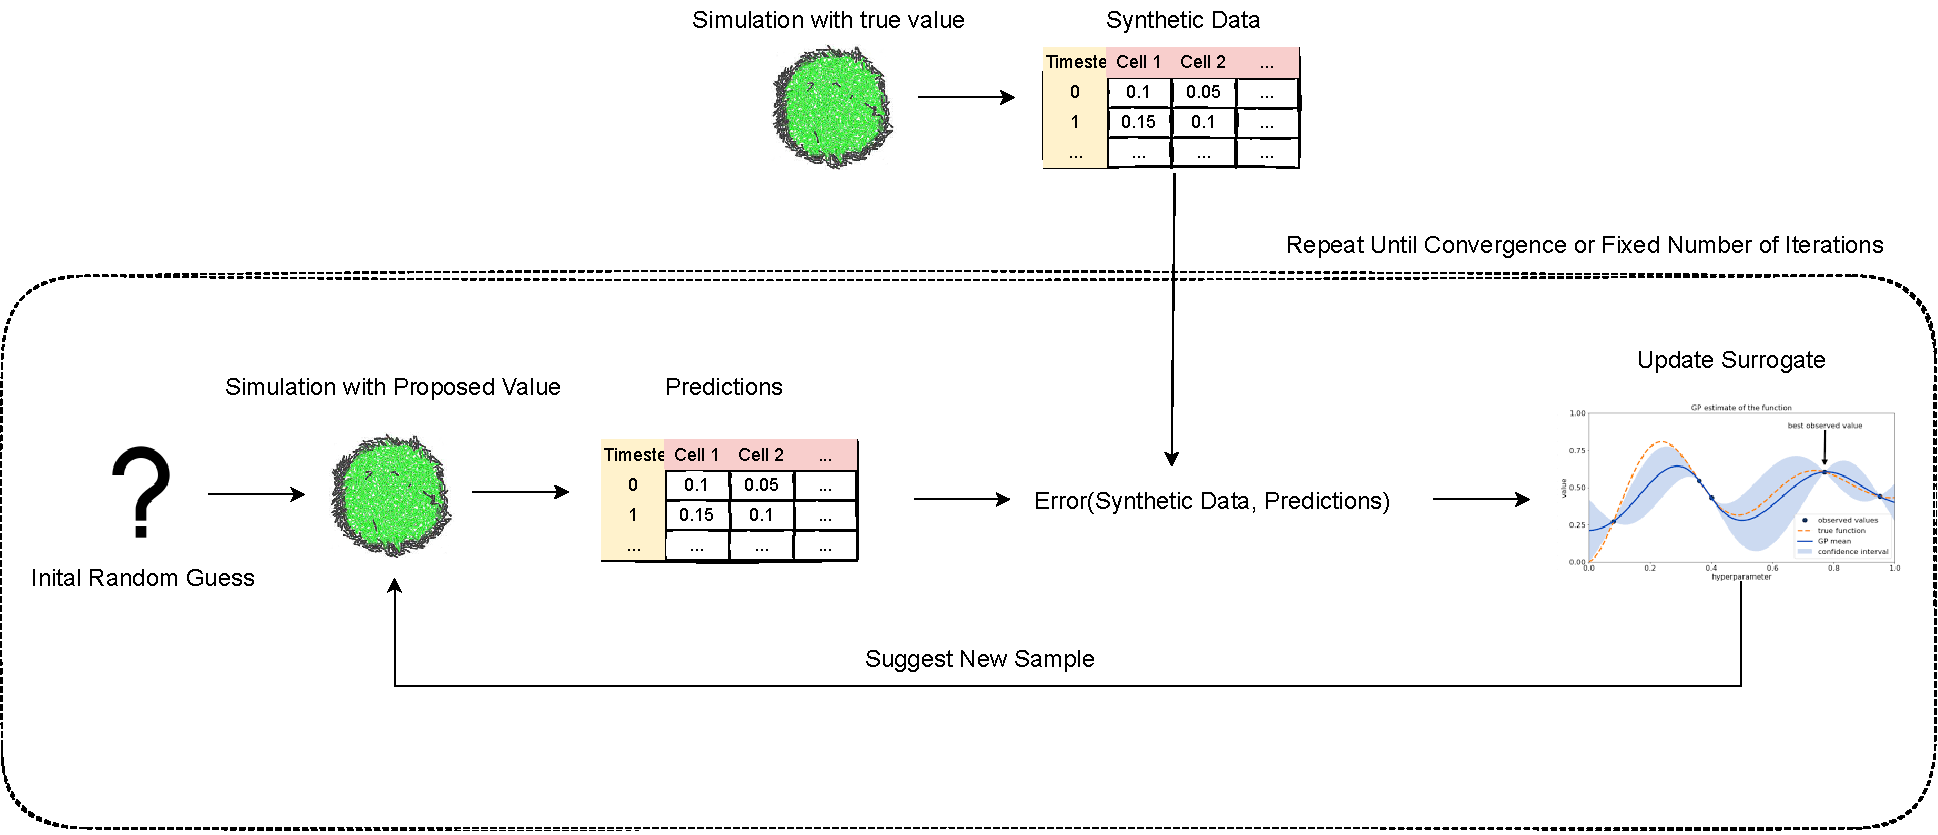
\includegraphics[width=0.95\textwidth]{Images/Other/Pipeline.pdf}
    \caption{Schematic representation of the pipeline adopted throughout the experiments. Firstly, the synthetic data is produced by using the true values of the parameters: this is the ground truth. Then, starting from an initial random guess, BayesOpt uses the error computed between predictions and synthetic data to refine its surrogate and propose new samples based on the acquisition function. The loop is repeated until the convergence criterion is met.}
    \label{fig:pipeline}
\end{figure}

I have used the experimental setup described to test the efficacy of BayesOpt under different conditions: increasingly large sampling spaces (Section \ref{sec:sampling_range}), noisy function evaluations (Section \ref{sec:noise}), and multiple parameters to infer simultaneously (Section \ref{sec:multiple}).

\subsection{Effects of Sampling range on Inference}\label{sec:sampling_range}

Biological parameters can often vary over several orders of magnitude, which increases the search space of viable parameter values \cite{pmid15369668}. By allowing parameters to vary over large ranges, biological systems develop the 'robustness' described in Section \ref{sec:systems_synth_bio} to survive against changing environmental conditions \cite{pmid21920040}. For this reason, I performed a series of experiments to systematically test the efficacy of BayesOpt in inferring parameters within variable-sized search spaces. 

I selected one key parameter of the ODE system and run a simulation for each sampling range with value $10^{x}$ for $x \in [1, 1.5, 2.0, 3.0, 3.5, 4.0]$. This means that for a sampling range value of $10^2$, for instance, the search space for the parameter $n$ extends from $n-100$ to $n+100$. Additionally, there is cut-off on the lower bound at zero, as biochemical rates are constrained to non-negativity. The BO algorithm runs until convergence, which I have manually defined to be met when the last 10 samples are all within 0.1 of the nominal value of the parameter. I repeat each experiment five times to to obtain an average result and observe any differences across runs. Results for this set of experiments are presented in Section \ref{sec:results_range}.

\subsection{Effect of Noisy Evaluations on Inference}\label{sec:noise}
Noise permeates biology on all levels, from the most basic molecular, sub-cellular processes to the dynamics of tissues, organs, organisms and populations \cite{tsimring2014noise}. At a molecular level, control strategies based on dynamic equilibrium of stochastic events have been shown to offer robustness and tunability in processes such as mRNA translation \cite{10.3389/fgene.2014.00052, doi:10.1126/science.1242975}. At a higher level, regulatory networks alter their topology to contribute to higher adaptability to changing environments and external noise (the 'robustness' property described in Sections \ref{sec:systems_synth_bio} and \ref{sec:sampling_range}). Although connections between noise at these different levels are still to be elucidated, there is strong evidence for its importance in the evolutionary process \cite{pmid18319722}. For this reason, I have conducted parameter inference via BayesOpt with different levels of artificial noise added to the simulated data. Note that an element of stochasticity is already present in the simulation itself, however an additional noise term could represent, for instance, external factors such as the microscope measurement error. 


The amount of noise introduced is defined by the Signal-to-Noise Ratio (SNR) \cite{johnson2006signal}. The SNR is the ratio of the signal power (in this context the concentration of the LacI protein) to the noise power:

\begin{equation}\label{eq:SNR}
    SNR = \frac{P_{signal}}{P_{noise}}
,\end{equation}

It is often expressed in decibels in the general context of signal processing. A ratio greater than 1:1 (or 0 dB) indicates more signal than noise. In order to add noise to the data, I first obtain the 'power of the signal', which for a random variable $X$ is equal to $E[X^{2}]$, where $E$ represents the expected value, or mean. In our case, this is the average concentration of LacI across all cells at time $t$

\begin{equation}\label{eq:P_signal}
    P_{signal} = E[(\text{LacI concentration at time $t$})^{2}],
\end{equation}

Since dB are used in the context of SNR, I convert the raw signal power to dB according to the following formula:

\begin{equation}
    P_{signal, dB} = 10log_{10}(P_{signal}),
\end{equation}

In a similar manner, 

\begin{equation}
    SNR_{dB} = 10log_{10}(SNR),
\end{equation}

and when we substitute \ref{eq:SNR} in the above, together with the quotient rule for logarithms, we obtain

\begin{equation}\label{eq:SNR_dB}
    SNR_{dB} = 10log_{10}(P_{signal}) - 10log_{10}(P_{noise}).
\end{equation}

I then provide a desired value of SNR in dB and use \ref{eq:SNR_dB} to obtain the desired amount of noise power. For the same reasoning in \ref{eq:P_signal}, this is equal to $E[(noise)^{2}]$. In turn, $E[(noise)^{2}] = \mu_{noise}^{2} + \sigma_{noise}^{2}$ \cite{durrett2019probability} which, if we assume that the noise has mean of 0, reduces to $\sigma_{noise}^{2}$, its variance. Noise is finally sampled from a Gaussian distribution centered at zero with standard deviation $\sigma_{noise}$ and added to the data produced by the simulation.

I have chosen SNR as a way to introduce noise because, by definition, it takes into account the values of the data the simulation produces, rather than blindly sampling gaussian noise with a prespecified standard deviation. This means that the method can easily be adapted to any other quantities one wished to perform parameter inference on without any fine-tuning required.

A visual representation of how much noise corresponds to different values of SNR is shown in Figure \ref{fig:noise}.

\begin{figure}[h]
    \centering
    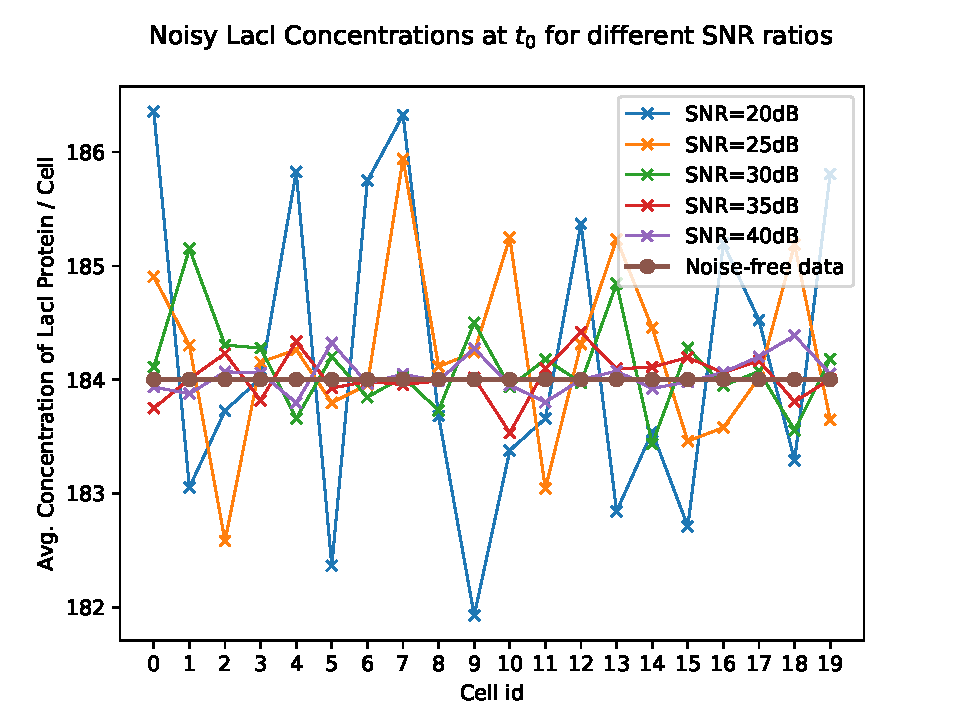
\includegraphics[width=0.8\textwidth]{Images/Noise/noisy_data.pdf}
    \caption{Gaussian noise is added to the average concentration of LacI protein in each cell for each timestep. The noise is sampled starting from a Signal-to-Noise (SNR) ratio, as described in equations \ref{eq:SNR} - \ref{eq:SNR_dB}.}
    \label{fig:noise}
\end{figure}

The convergence criterion I initially adopted for this set of experiments was the same described in Section \ref{sec:sampling_range}, i.e. sampling for 10 consecutive iterations within 0.1 of the nominal value of the parameter. However, I found that BayesOpt would never meet the criterion and therefore terminate. The first step I took towards a solution was relaxing the convergence criterion, which did not lead to any improvements. This suggested that the problem could lie within the hyperparameter settings of the BayesOpt algorithm itself. Based on this insight, I modified the acquisition function from Expectation Improvement (EI), to Noisy Expectation Improvement (NEI), as proposed in \cite{https://doi.org/10.48550/arxiv.1706.07094}. The main issue with EI is that it computes the next sample based on the best function evaluation so far, which becomes challenging in a noisy setting given that the best estimate is unreliable. The authors of \cite{https://doi.org/10.48550/arxiv.1706.07094} provide compelling evidence for how NEI outperforms both EI and various heuristics used in combination with EI to deal with noise. The GPyOpt library does not support NEI, however I found a partially working implementation at \cite{NEI} which I used as a starting point to integrate with the other modules in the library and overall pipeline. NEI allowed BayesOpt to terminate for the 40dB SNR experiment, however noise levels from 35dB to 20dB would still pose problems. Therefore, I modified the convergence criterion altogether, by running BayesOpt for a fixed number of iterations and observing the frequency counts of the sampled values. This choice was also dictated by the fact that NEI is significantly slower than EI, and I could not afford to let the experiments run for large number of iterations due to time and computational constraints under which this work has been carried out.

Results for this set of experiments are presented in Section \ref{sec:results_noise}.

\subsection{Effects of Multiple Variables on Inference}\label{sec:multiple}
A common difficulty encountered in parameter inference is that the model equations usually have a large number of unknowns, which cannot be determined individually with reasonable accuracy due to correlations between the parameters \cite{pmid19215296, pmid18817540}. Moreover, as already mentioned in Section \ref{sec:sampling_range} and as shown by Gutenkunst \textit{et al.} \cite{pmid17922568}, multiple parameterizations can reflect the model behaviour, with some parameters being 'stiff' (accurately identifiable) and others being 'sloppy' (varying by orders of magnitude without significantly influencing the quality of the fit). On the other hand, one could argue that often the precise value of a parameter is not required to draw biological conclusions \cite{pmid18817540}. I therefore considered testing BayesOpt inference with multiple parameters important.

Inference of two parameters successfully terminates according to the convergence criterion defined in Section \ref{sec:sampling_range}. When inferring three and four variables, however, I had to modify the convergence criterion for the algorithm to terminate, similarly to the experiments described in Section \ref{sec:noise}. This was not done due to noisy function evaluations, however, but for the identifiability problem of sloppy parameters described above, as well as the toll imposed by the curse of dimensionality \cite{kuo2005lifting}: the prohibitive rise in computational costs due to the exponential growth of the search space as the number of parameters increases.

Results for this set of experiments are presented in Section \ref{sec:results_multiple}.


\subsection{Biological Model}\label{sec:biological_model}
The simulation I chose to use throughout the experiments models a 'synthetic biological clock' in populations of \textit{E. Coli} \cite{doi:10.1073/pnas.0307095101}. Bacterial populations exhibit diverse biochemical rhythms, behaviours that repeat themselves by following regular patterns. These arise from the synchronous coordination of the individual cells' oscillations.

The reason I chose this particular model is that it is contained in the bsim installation files, therefore allowing me to avoid implementing the bio-chemical details. I still had to modify the source code to log the relevant data and interface bsim with the BayesOpt module. Initially, I started to implement the model described in Section \ref{sec:theory_abm}, representing allocation of finite resources by molecular processes. However, due to time constraints and the fact the core topic of the project is Bayesian Optimization, rather than any specific biological model, I decided to forgo the idea to speed up development.

The biological clock model is described by seven ODEs and six parameters (equations \ref{eq:model_first} - \ref{eq:model_last}). The nominal values of the parameters are reported in Table \ref{tab:model_params}.

\begin{equation}\label{eq:model_first}
    \frac{da_{i}}{dt} = -a_{i} + \frac{\alpha}{1+C_{i}^{n}},
\end{equation}

\begin{equation}\label{}
    \frac{db_{i}}{dt} = -b_{i} + \frac{\alpha}{1+A_{i}^{n}},
\end{equation}

\begin{equation}\label{}
    \frac{dc_{i}}{dt} = -c_{i} + \frac{\alpha}{1+B_{i}^{n}} + \frac{kS_{i}}{1+S_{i}},
\end{equation}

\begin{equation}\label{}
    \frac{dA_{i}}{dt} = \beta (a_{i} - A_{i}),
\end{equation}

\begin{equation}\label{}
    \frac{dB_{i}}{dt} = \beta (b_{i} - B_{i}),
\end{equation}

\begin{equation}\label{}
    \frac{dC_{i}}{dt} = \beta (c_{i} - C_{i}),
\end{equation}

\begin{equation}\label{eq:model_last}
    \frac{dS_{i}}{dt} = -k_{s0}S_{i} + k_{s1}A_{i} - \eta(S_{i} - S_{e}).
\end{equation}

For the biological meaning of the equations and parameters, I refer to the original work in which the model was presented \cite{doi:10.1073/pnas.0307095101}.

\begin{table}[t]
    \centering
    \begin{tabular}{cc}
    \toprule[1pt]
        \textbf{Name}  & \textbf{Value} \\ \hline
        $\alpha$ & 216.0 \\
        $n$ & 2.0 \\
        $\eta$ & 2.0 \\
        $k_{s0}$ & 1.0 \\
        $k_{s1}$ & 0.01 \\
        $\kappa$ & 20.0 \\
    \bottomrule[1pt]
    \end{tabular}
    \caption{Nominal values of the parameters for the model presented in \cite{doi:10.1073/pnas.0307095101}. These represent the 'true values' used to obtain the synthetic data, or ground truth, used by BayesOpt top update the surrogate.}
    \label{tab:model_params}
\end{table}

I let the model run for 10 (simulated) seconds. This value has been determined empirically to strike a balance between complexity of the data collected and speed when run multiple times throughout BayesOpt. I leave for future research the task of running the simulation for longer and performing parameter inference on vaster datasets.



\chapter{Results}\label{ch:results}
This chapter presents the results of the experiments illustrated in Chapter \ref{ch:experiments}. Bayesian Optimization is shown to provide accurate estimates when sampling from increasingly large sampling spaces, while struggling when gaussian noise is added to the function evaluations. It correctly infers simultaneously two parameters, whereas for three and four parameters it is difficult to asses its efficacy due to the  limited iterations the algorithm was run for.  

\section{Effects of Sampling Range on Inference}\label{sec:results_range}
Bayesian Optimization has been adopted to infer parameters from an increasingly large sampling space following the considerations in Section \ref{sec:sampling_range}. I have arbitrarily chosen $\kappa$, with nominal value of 20.0, to be inferred. The convergence criterion is met when the last 10 proposed samples are all within 0.1 of the nominal value of the parameter. The acquisition function used is expectation improvement. Five experiments are run for each sampling range and the results averaged.

Figure \ref{fig:progression} illustrates the progression of the algorithm. Table \ref{tab:range_table} and Figure \ref{fig:range_iters} summarise the results.

The number of iterations needed to converge increases as the sampling space expands. The average number of iterations, computed over the five runs of each set of experiments, stays stable between $10^{1}$ and $10^{2}$, while showing a 5-fold increase from $10^{2}$ and $10^{3}$, and a 1.5 increase to $10^{4}$. I could not identify any clear trend in the relationship between iterations and range due to the limited size of the data. However, these initial results are promising as for practical applications, in which prior knowledge about the parameter by the modeller can further reduce the search space, successfully sampling over a range of $\pm 10^{4}$ is good enough. A more through analysis would include sampling over even vaster ranges as well as repeating each set of experiments for a greater number of times to obtain more statistically significant results. However, due to computational and time constrains encountered during this work, it is left up to future research. 

The standard deviation across experiment sets rises at a much faster rate. This can be observed in Figure \ref{fig:range_iters}, where a Gaussian distribution has been fitted to each set of experiments and appears to capture the variability of the individual data points. This can be explained by the fact that the algorithm has fewer chances of sampling in the vicinity of the minimum early on, given the vastness of the search space.

\begin{table}[h]
    \centering
    \begin{tabular}{ccc} \toprule
        \textbf{Range} ($\mathbf{\pm 10^{x}}$) & \textbf{Average} & \textbf{Standard Deviation} \\ \hline
        1.0 & 13 & 1.41 \\
        1.5 & 13 & 0.97 \\
        2.0 & 15 & 3.57 \\
        2.5 & 32 & 13.04 \\
        3.0 & 82 & 32.98 \\
        3.5 & 90 & 35.00 \\
        4.0 & 126 & 86.98 \\
    \end{tabular}
    \caption{Number of iterations (average and standard deviation for five runs of each experiment) needed for BayesOpt to converge to the nominal value of $\kappa = 20 \pm 0.1$ when sampling search spaces of different sizes.}
    \label{tab:range_table}
\end{table}

\begin{figure}[h]
    \centering
    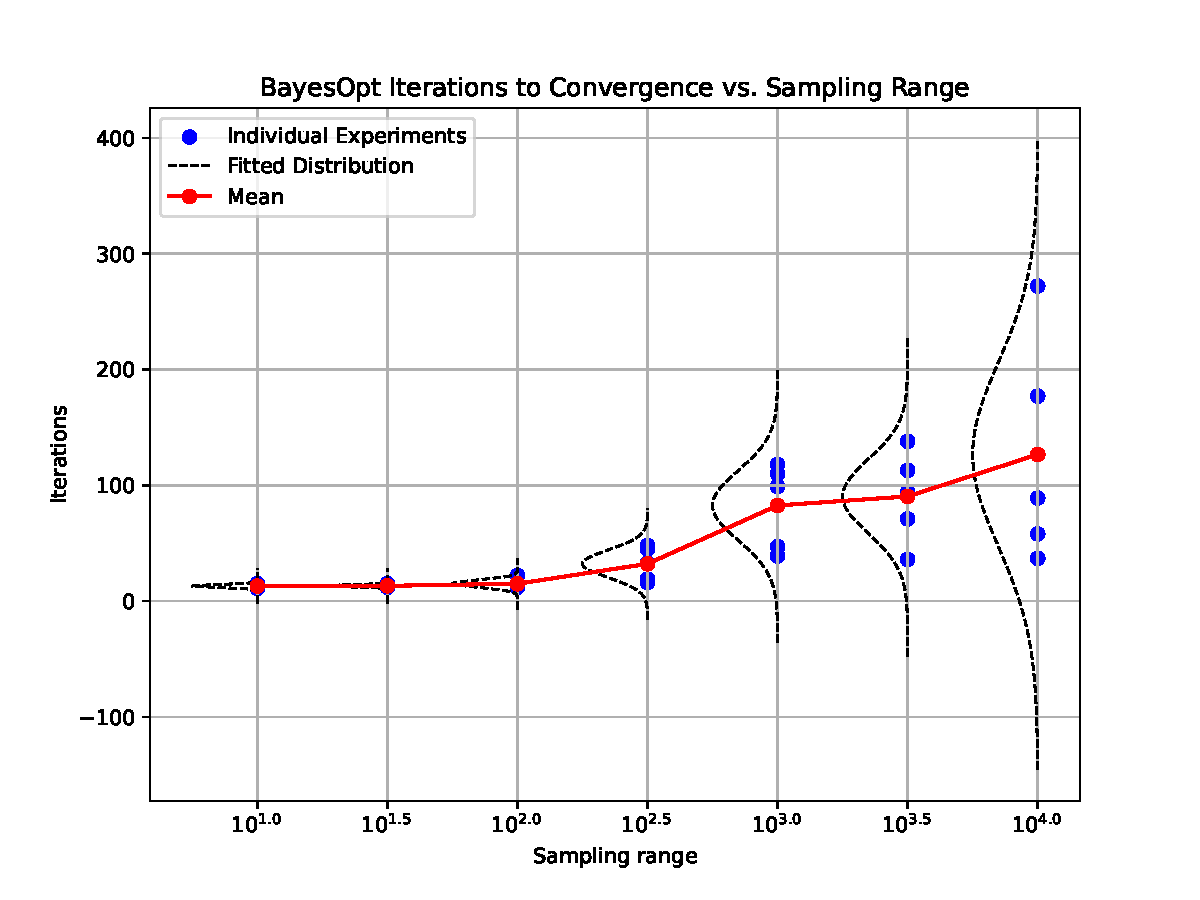
\includegraphics[width=0.6\textwidth]{Images/Range/ranges_iters.pdf}
    \caption{Number of iterations needed for BayesOpt to converge to nominal value of $\kappa = 20 \pm 0.1$ when sampling search spaces of different sizes. Both individual experiments and averages are shown. Note the increase in iterations as the sampling space expands, as well as the higher variability in the number of iterations required. The number of iterations required for each sampling range is normally distributed.}
    \label{fig:range_iters}
\end{figure}


% Position figure exactly at top of the page %
\makeatletter
\setlength{\@fptop}{0pt}
\makeatother

\begin{figure}[ht]
    \centering
    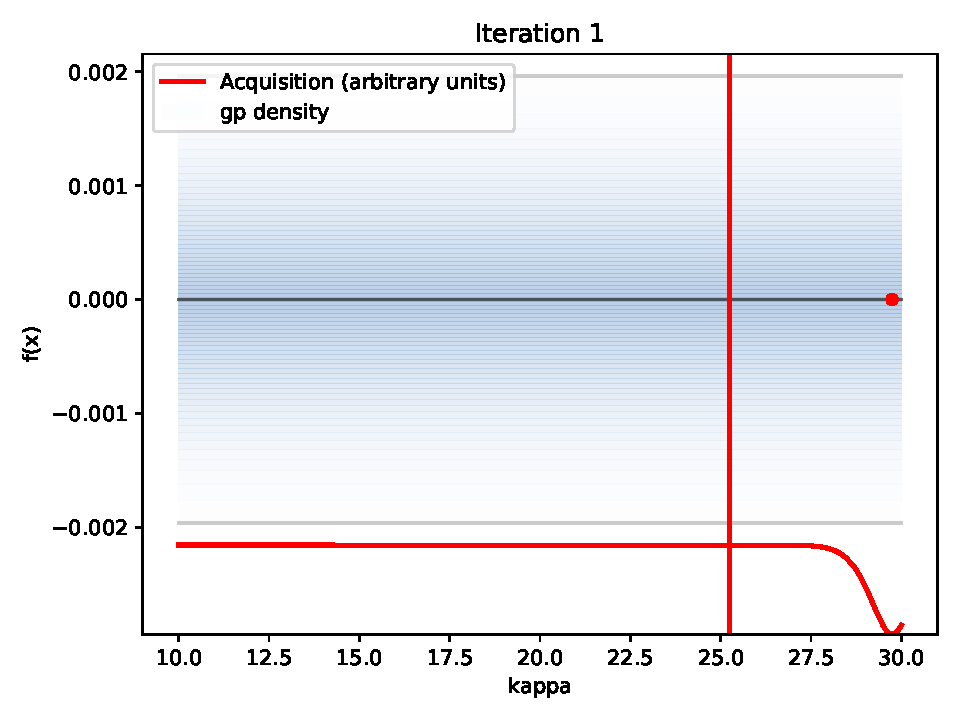
\includegraphics[width=.25\textwidth]{Images/Range/convergence_iter_1.pdf}
    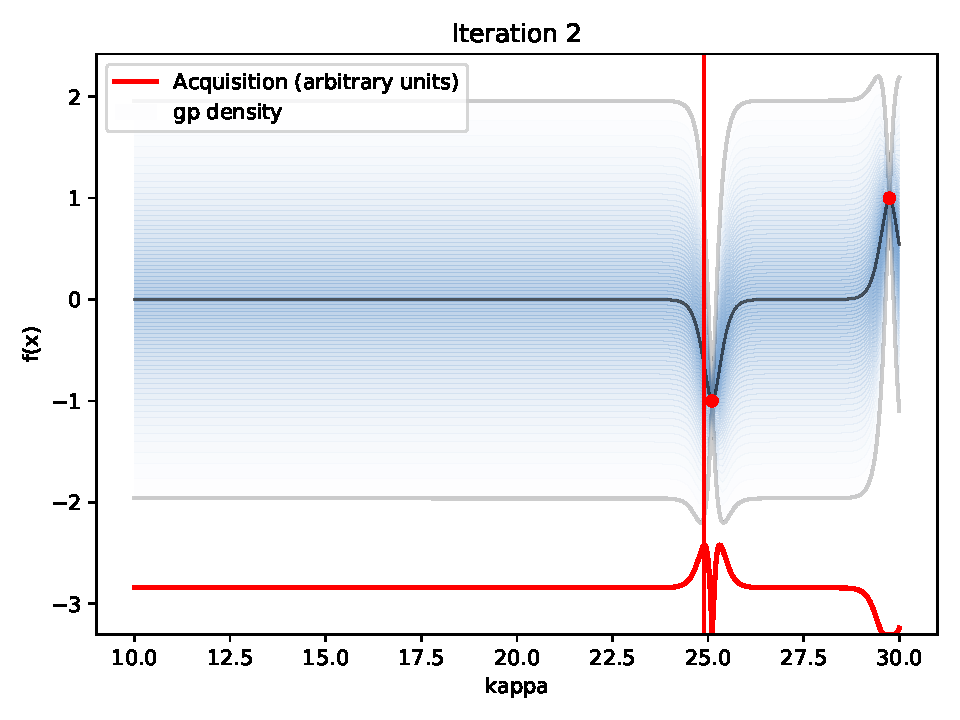
\includegraphics[width=.25\textwidth]{Images/Range/convergence_iter_2.pdf}
    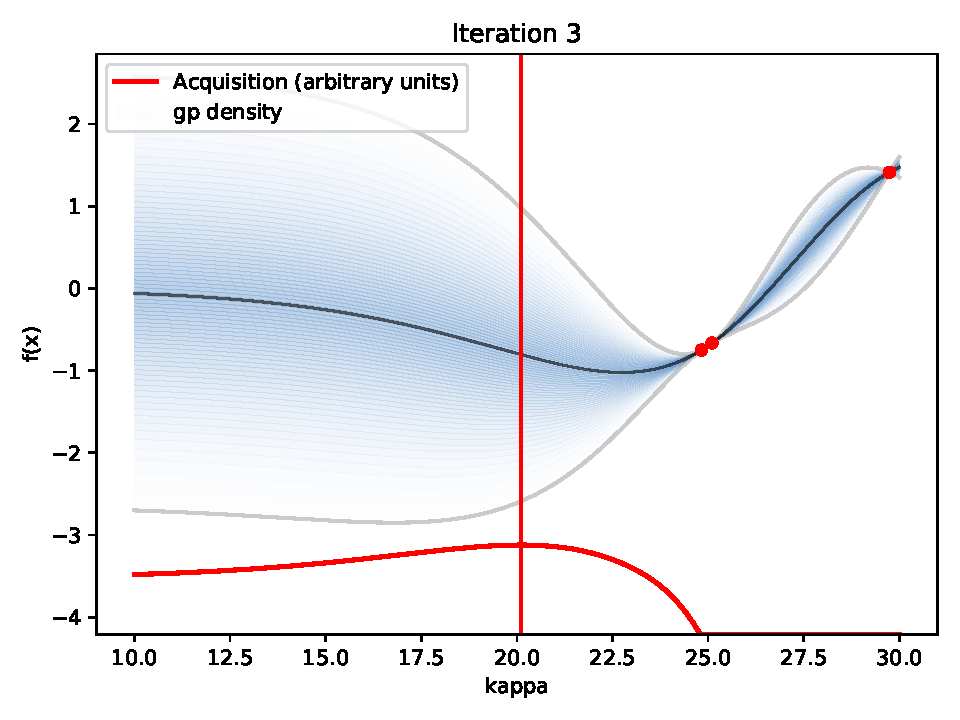
\includegraphics[width=.25\textwidth]{Images/Range/convergence_iter_3.pdf}
    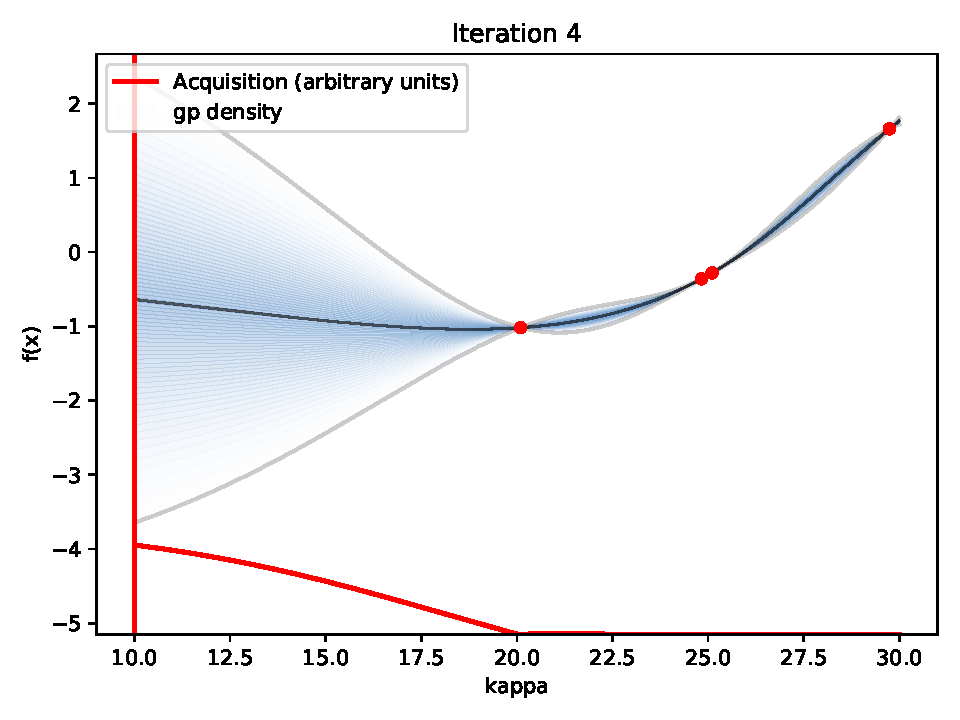
\includegraphics[width=.25\textwidth]{Images/Range/convergence_iter_4.pdf}
    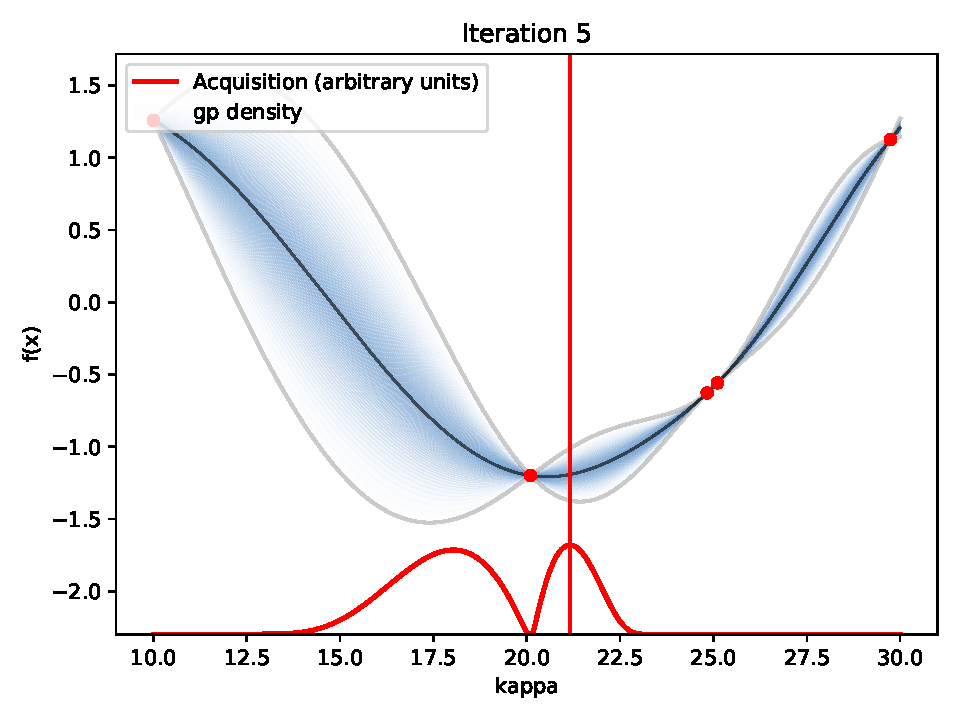
\includegraphics[width=.25\textwidth]{Images/Range/convergence_iter_5.pdf}
    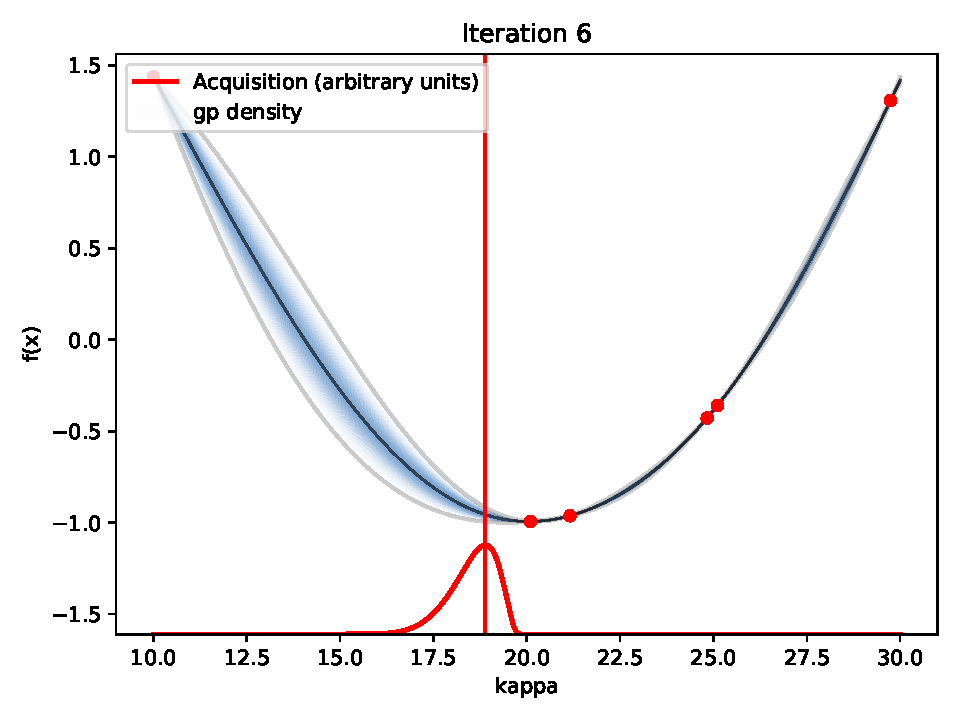
\includegraphics[width=.25\textwidth]{Images/Range/convergence_iter_6.pdf}
    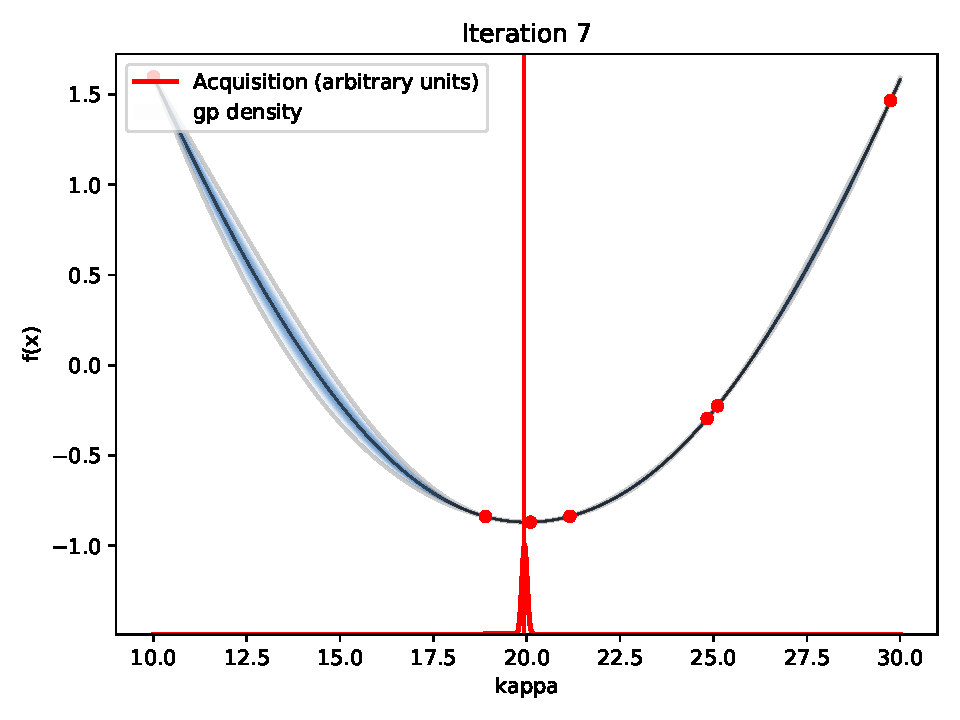
\includegraphics[width=.25\textwidth]{Images/Range/convergence_iter_7.pdf}
    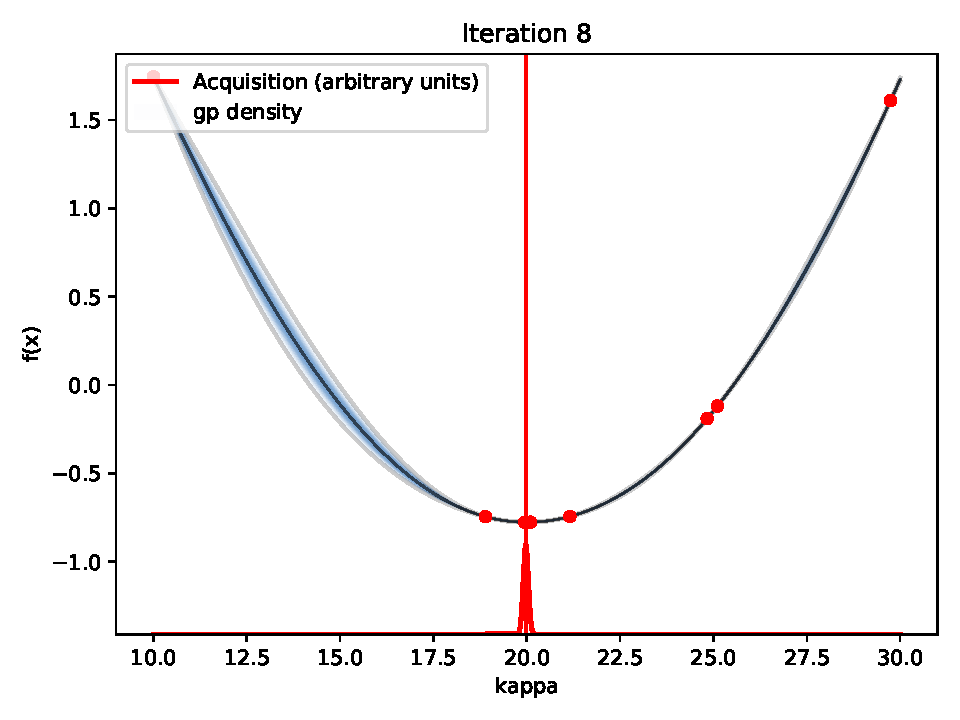
\includegraphics[width=.25\textwidth]{Images/Range/convergence_iter_8.pdf}
    \caption{BayesOpt inference of $\kappa$ (nominal value = 20.0), with sampling space $\pm$10, expected improvement as acquisition function, starting point randomly chosen in $[\kappa-10, \kappa+10]$, and no noise added to the function evaluations. The figure shows the surrogate (black), the confidence intervals (shaded blue), and the acquisition function (red). At each iteration the value of $\kappa$ that maximizes the acquisition function is chosen as the next sampling point, the simulation is run with that value and the error computed between the simulated data and the synthetic data is used to update the surrogate.}
    \label{fig:progression}
\end{figure}




\section{Effects of Noisy Evaluations on Inference}\label{sec:results_noise}
Bayesian Optimization has been adopted to infer parameters with gaussian noise added to the function evaluations, following the considerations in Section \ref{sec:noise}. I have arbitrarily chose $\kappa$ to be inferred, with nominal value of 20.0, and a sampling space of $\pm$ 10. The algorithm would not converge according to the criterion adopted for the experiments in Section \ref{sec:results_range}, therefore BayesOpt is run for a fixed number of iterations (50) and the resulting sampling frequencies inspected.

As Figure \ref{fig:noise_histograms} illustrates, the algorithm successfully converges to the true value of the parameter with SNR = 40dB, with the sampled values appearing to be normally distributed. The estimates quickly start to deteriorate for increasing levels of noise, starting with SNR = 30dB. A possible explanation for this behaviour is that the noise levels are too high, therefore multiple function evaluations $f(x)$ will yield different results for the same $x$. This leads BayesOpt to keep sampling around the same $x$ multiple times until the uncertainty around that value is reduced, which is hard given the variability of the evaluations at that point. This explains why, for high levels of noise, there is a concentration of sampling around one or two values, whereas for SNR = 40dB the samples are more spread out. This hypothesis if further corroborated by Figure \ref{fig:noise_posteriors}, showing the posterior and acquisition functions, as well as the function evaluations at the proposed samples, for SNR = 40dB and SNR = 30dB. In the case of SNR = 40dB, we can already observe how the variability of the evaluations leads to many peaks in the acquisition functions, indicating that there a are still a number of areas the algorithm wishes to explore. From the overall shape of the posterior, however, it is clear that BayesOpt has a rough idea of where the minimum is (compare this with the noise-free posterior in Figure \ref{fig:progression}). In the case of SNR = 30 dB, however, the evaluations for the same $\kappa \approx 22.5$ yield significantly different values, leading to BayesOpt getting stuck.

There are a number of considerations to be made regarding the experiments. Note that these have not been implemented due to time and computational constraints and are left for future research.

\begin{enumerate}
    \item A SNR of 40dB might be enough in certain contexts; the levels of noise to be simulated are application-specific and fine-tuning is required by modellers;
    \item BayesOpt could be run for a number of iterations greater than 50. The panel in Figure \ref{fig:noise_histograms} corresponding to SNR = 35dB, for instance, shows that the algorithm has sampled in the vicinity of the true value, and a more accurate estimate could have been obtained given a greater number of iterations;
    \item My implementation of the NEI acquisition function requires more thorough testing to be confident of its efficacy;
    \item A number of other acquisition functions can deal with noisy evaluations, such as entropy search \cite{10.5555/2188385.2343701} and knowledge gradient \cite{doi:10.1137/100801275}. These have not been implemented and a thorough comparative analysis would be required to determine whether the problem lies with the type of acquisition rather than the levels of noise. 
\end{enumerate}


\begin{figure}[htb]
    \centering
    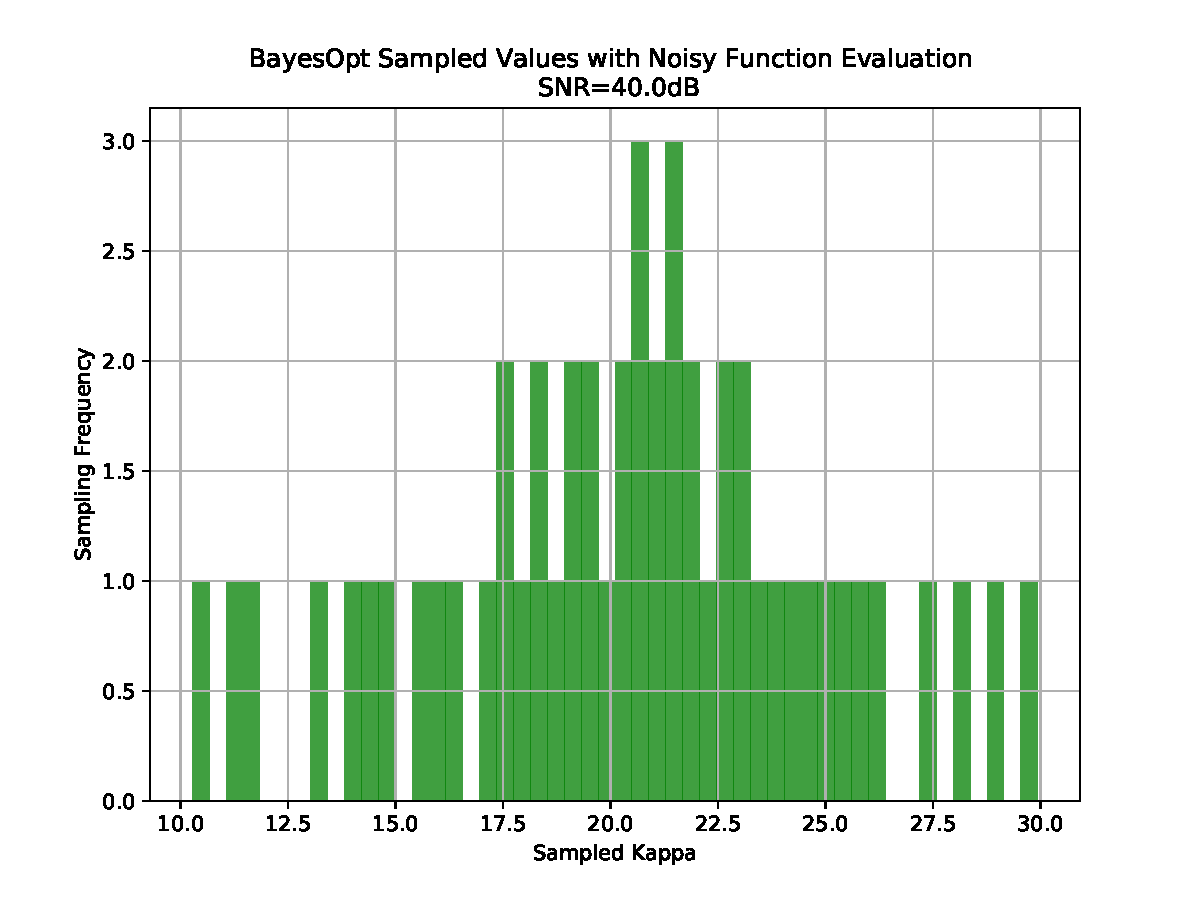
\includegraphics[width=0.3\textwidth]{Images/Noise/Histogram_Noise_40.0.pdf}
    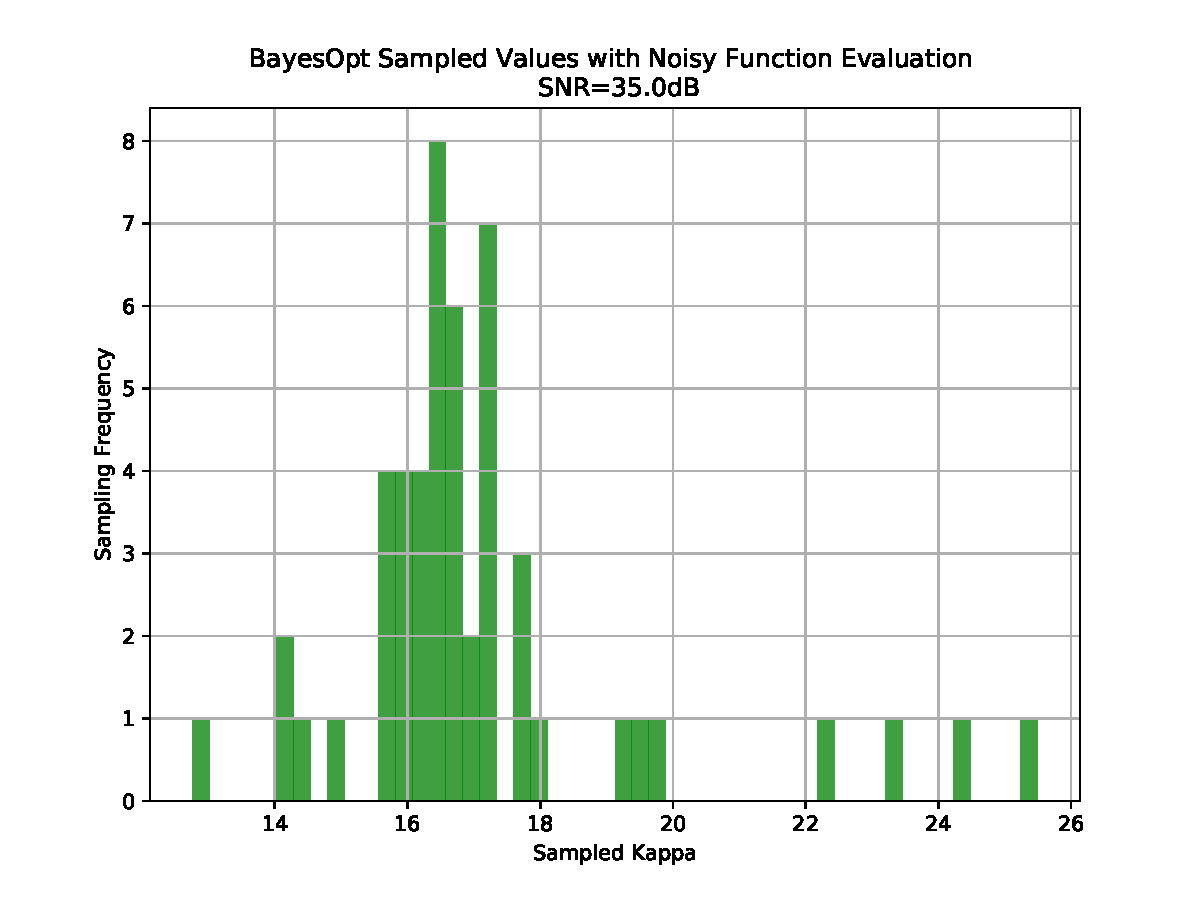
\includegraphics[width=0.3\textwidth]{Images/Noise/Histogram_Noise_35.0.pdf}
    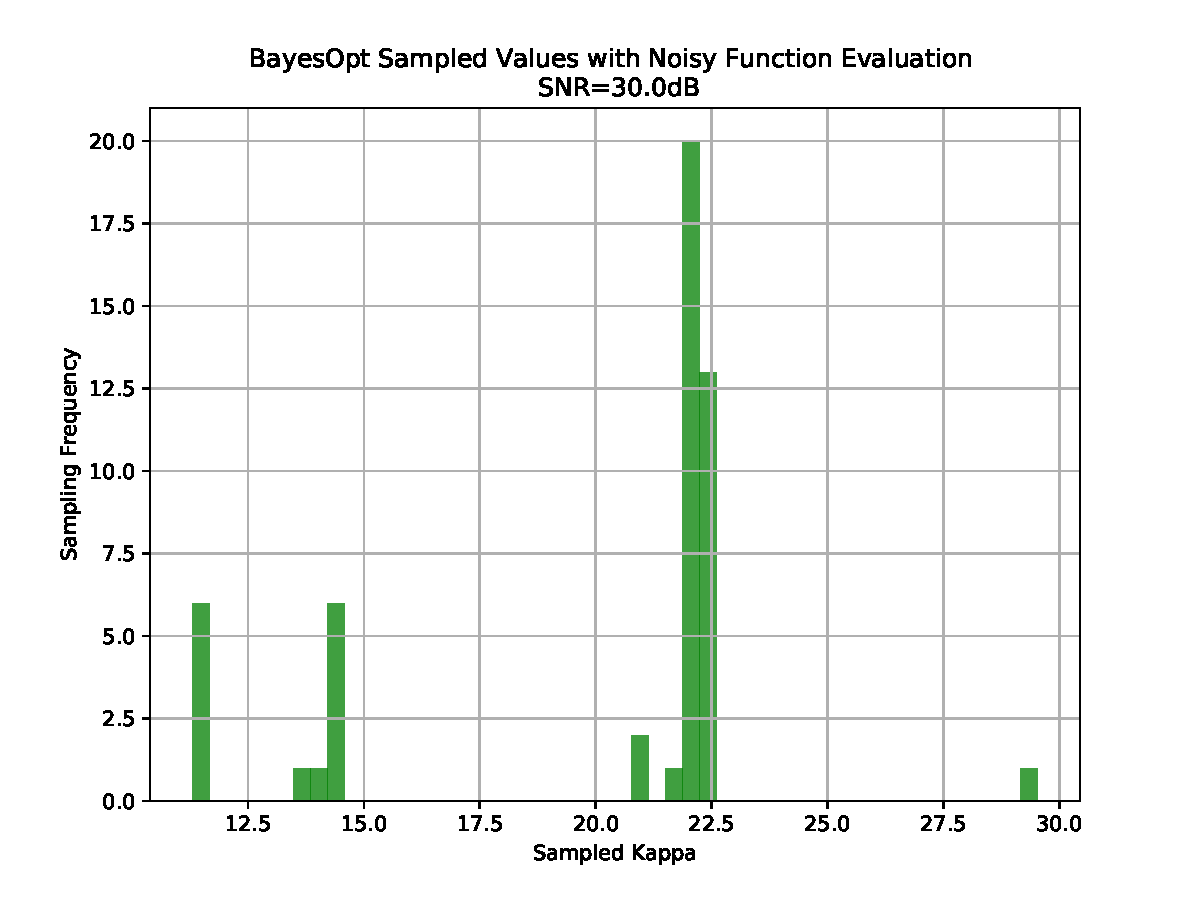
\includegraphics[width=0.3\textwidth]{Images/Noise/Histogram_Noise_30.0.pdf}
    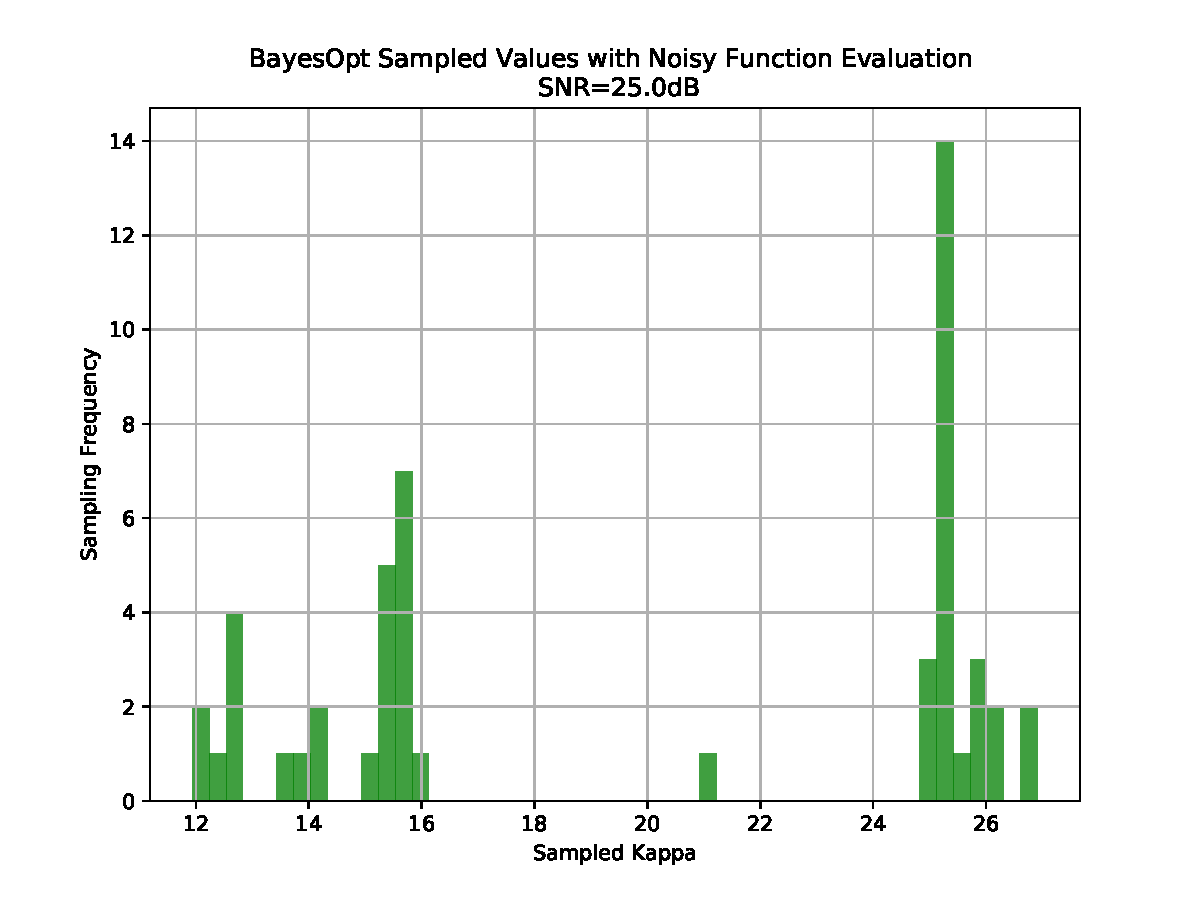
\includegraphics[width=0.3\textwidth]{Images/Noise/Histogram_Noise_25.0.pdf}
    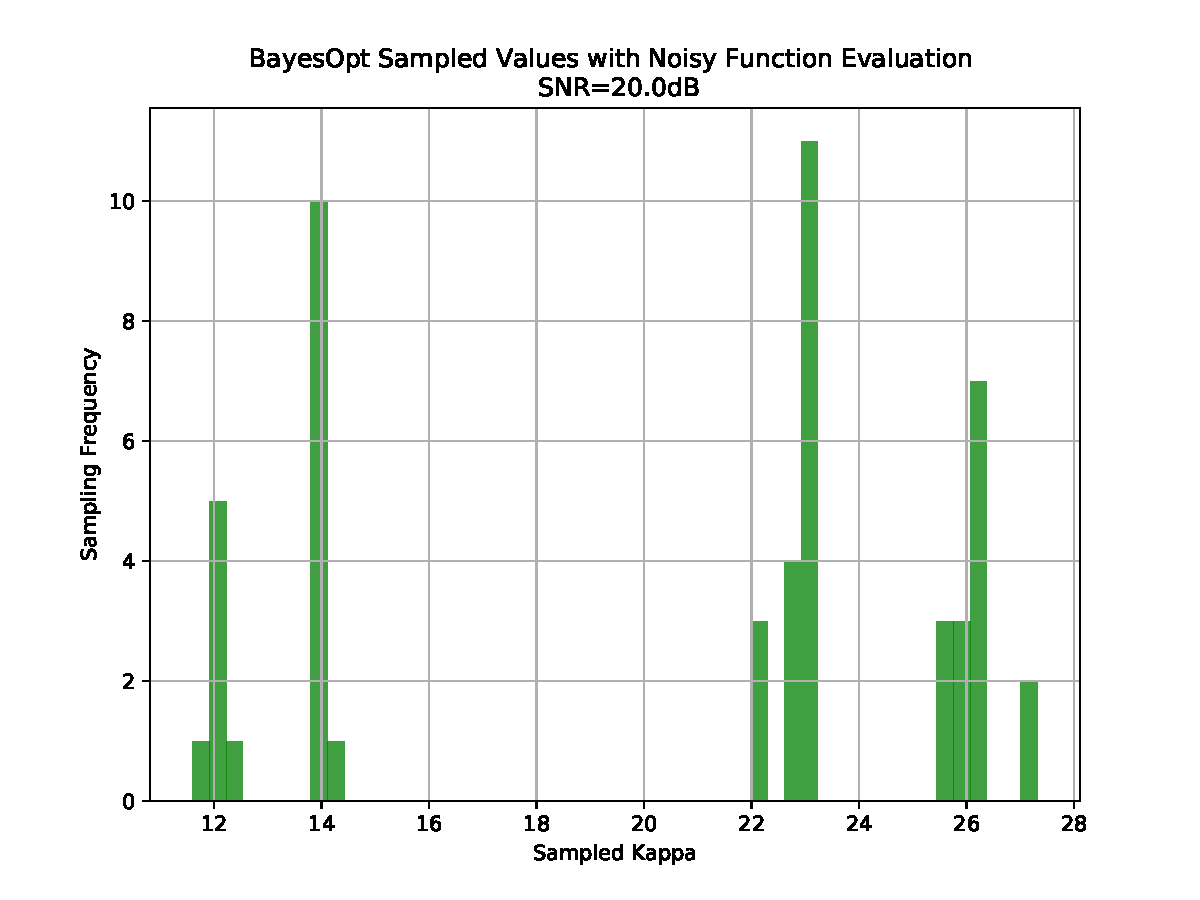
\includegraphics[width=0.3\textwidth]{Images/Noise/Histogram_Noise_20.0.pdf}
    \caption{Sampling frequency of BayesOpt-proposed values with Gaussian noise added to function evaluations. Noise is added based on Signal-to-Noise (SNR) ratio, as described in Section \ref{sec:noise}. Note how the parameter is correctly inferred with a SNR of 40dB, and estimates become progressively worse for greater levels of noise. }
    \label{fig:noise_histograms}
\end{figure}


\begin{figure}[htb]
    \centering
    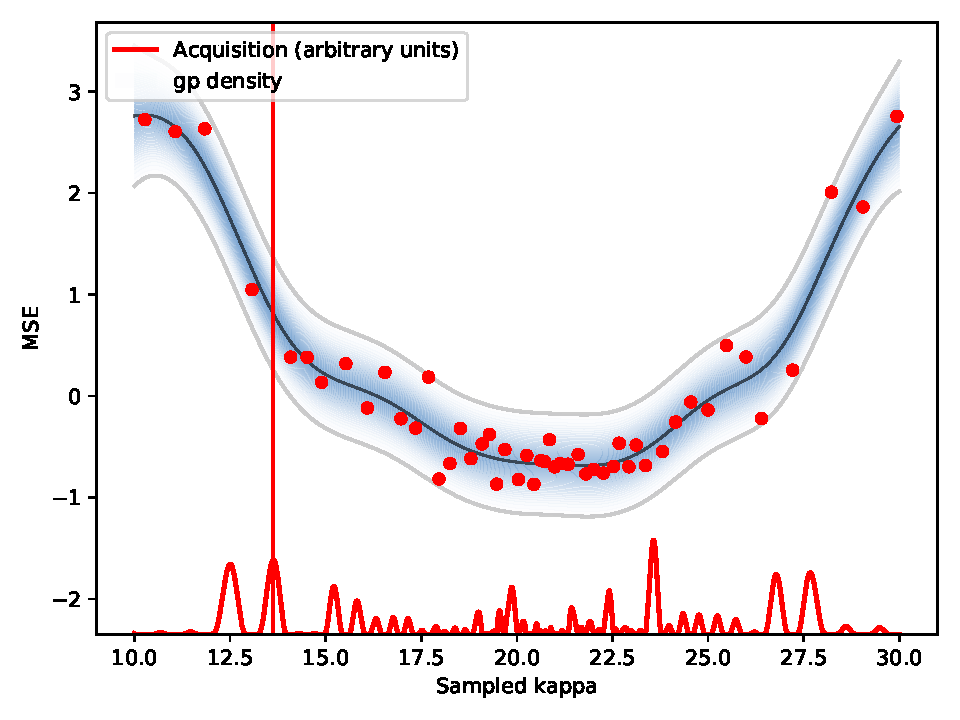
\includegraphics[width=0.45\textwidth]{Images/Noise/acquisition_noise40.pdf}  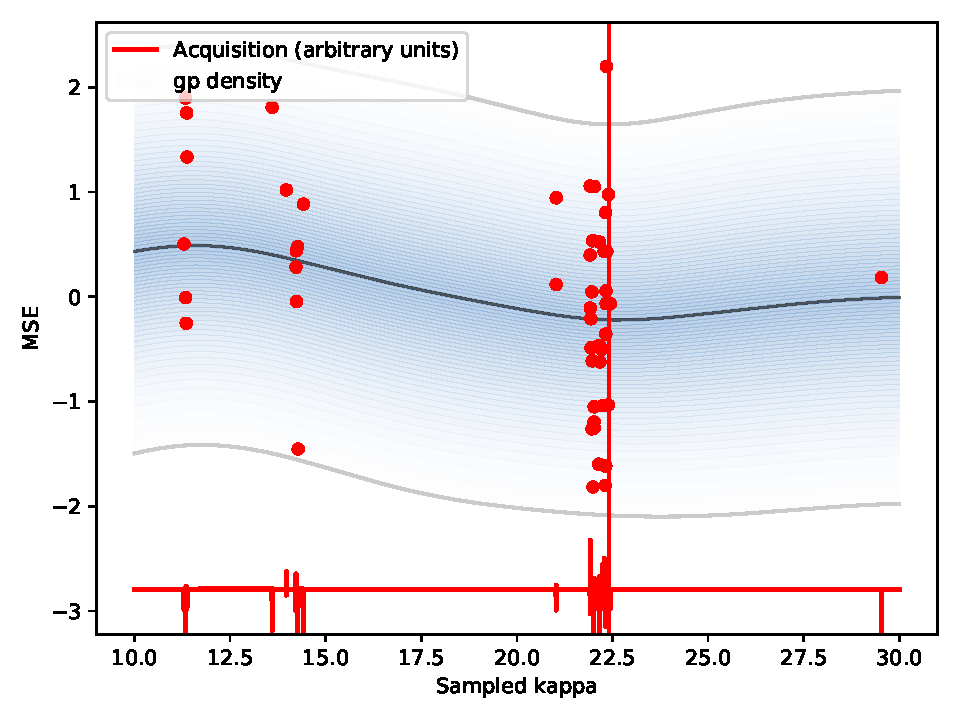
\includegraphics[width=0.45\textwidth]{Images/Noise/acquisition_noise30.pdf} 
    \caption{Surrogate and NEI acquisition function after 50 iterations with noisy evaluations. \textit{Left panel}: SNR=40dB; \textit{Right panel}: SNR=30dB.}
    \label{fig:noise_posteriors}
\end{figure}

\section{Effects of Multiple Variables on Inference}\label{sec:results_multiple}
Bayesian Optimization has been adopted to infer multiple parameters at the same time following the considerations in Section \ref{sec:multiple}. I have arbitrarily chosen the parameters to infer to be $k_{s0} = 1.0$, $\alpha=216.0$, $\kappa=20.0$, $nExp = 2.0$.

For two-parameter inference, the convergence criterion of sampling ten consecutive values within 0.1 of the nominal values of the parameters is successfully met by BayesOpt. A progression of the algorithm is shown in Figure \ref{fig:2var_progression}: although the objective function shows a 'valley' (area where the objective is uniformly low), BayesOpt is able to find the global minimum. Figure \ref{fig:2var_sampled_values} shows how the algorithm, after identifying the correct value of $\alpha$ around iteration 20, keeps this fixed and explores the 'valley' by varying $k_{s0}$. BayesOpt converges in around 30 iterations (experiments were repeated five times and results averaged).

\begin{figure}[h]
    \centering
    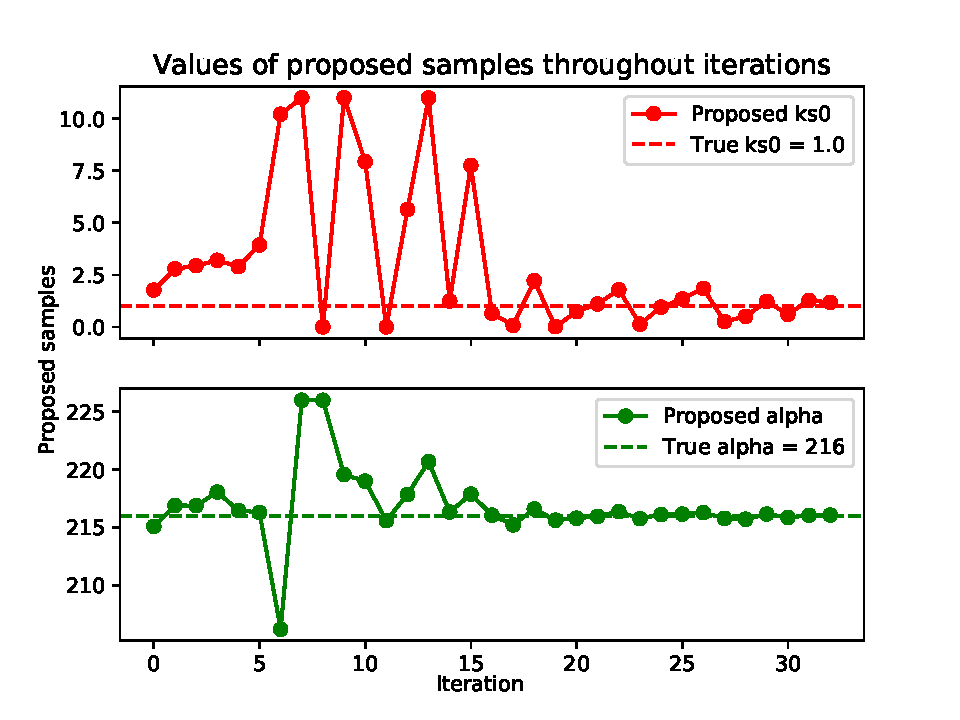
\includegraphics[width=0.7\textwidth]{Images/Multiple variables/Sample values_2var.pdf}
    \caption{Sampled values of $k_{s0}$ and $\alpha$ (nominal values 1.0 and 216.0, respectively) throughout iterations. The algorithm successfully terminates after roughly thirty iterations.}
    \label{fig:2var_sampled_values}
\end{figure}

\begin{figure}[ht]
    \centering
    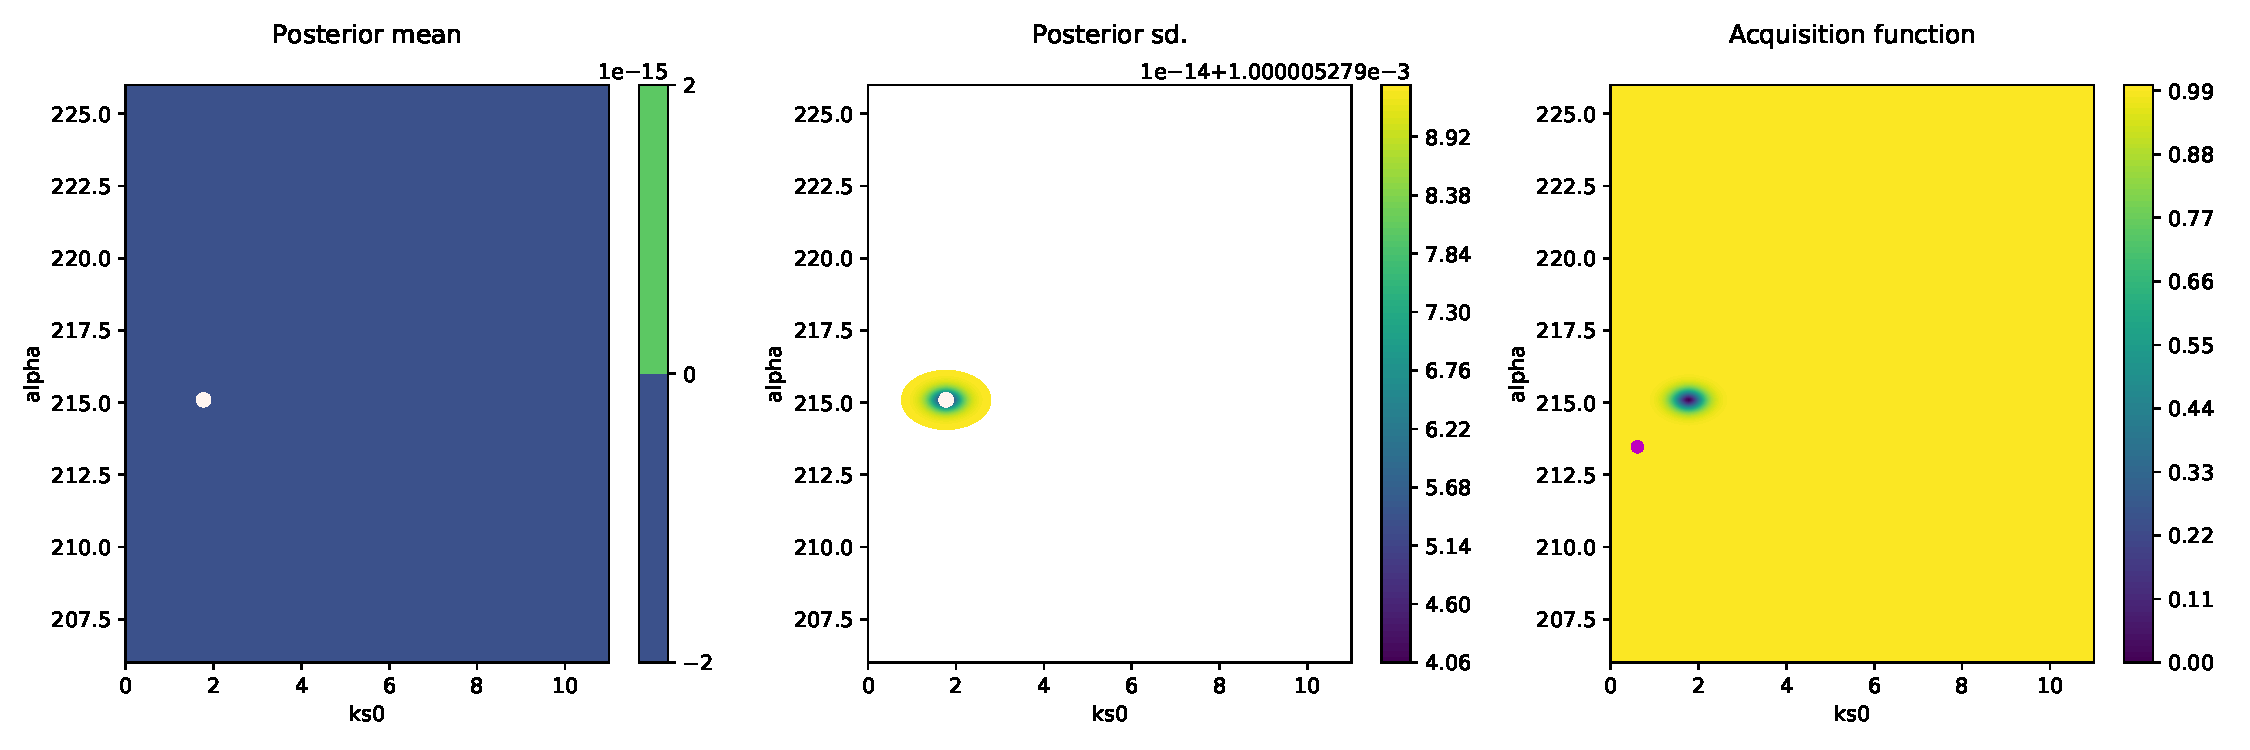
\includegraphics[width=0.7\textwidth]{Images/Multiple variables/2var_convergence_iter_1.pdf}
    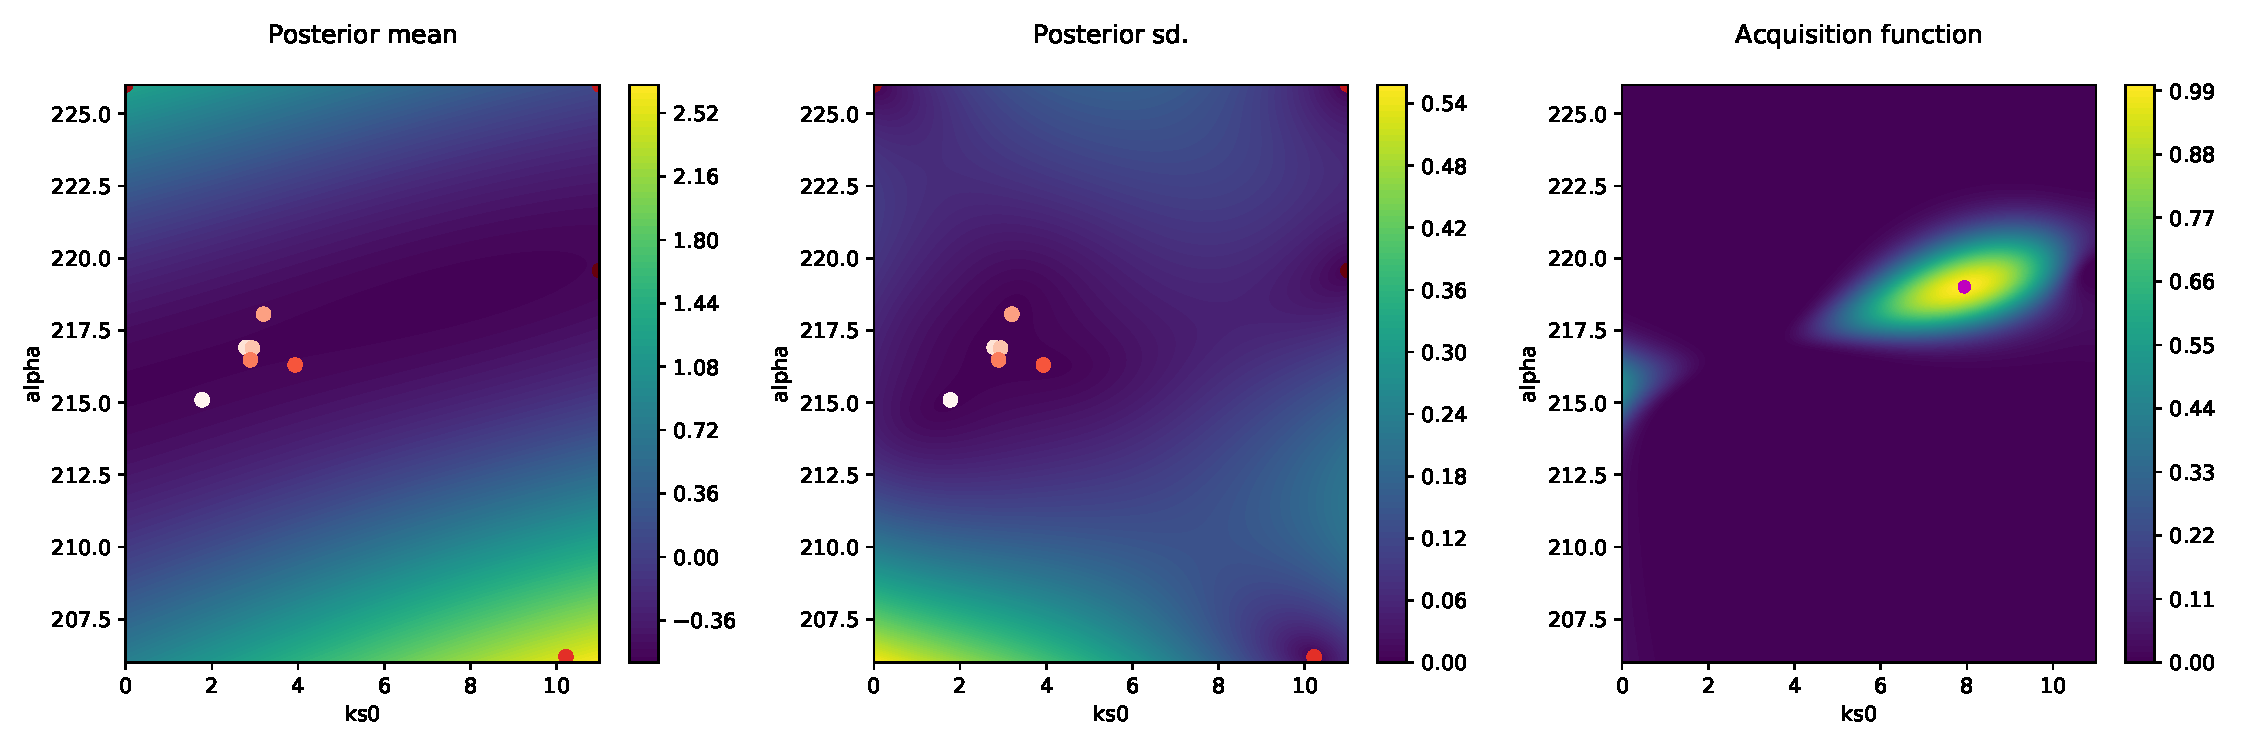
\includegraphics[width=0.7\textwidth]{Images/Multiple variables/2var_convergence_iter_10.pdf}
    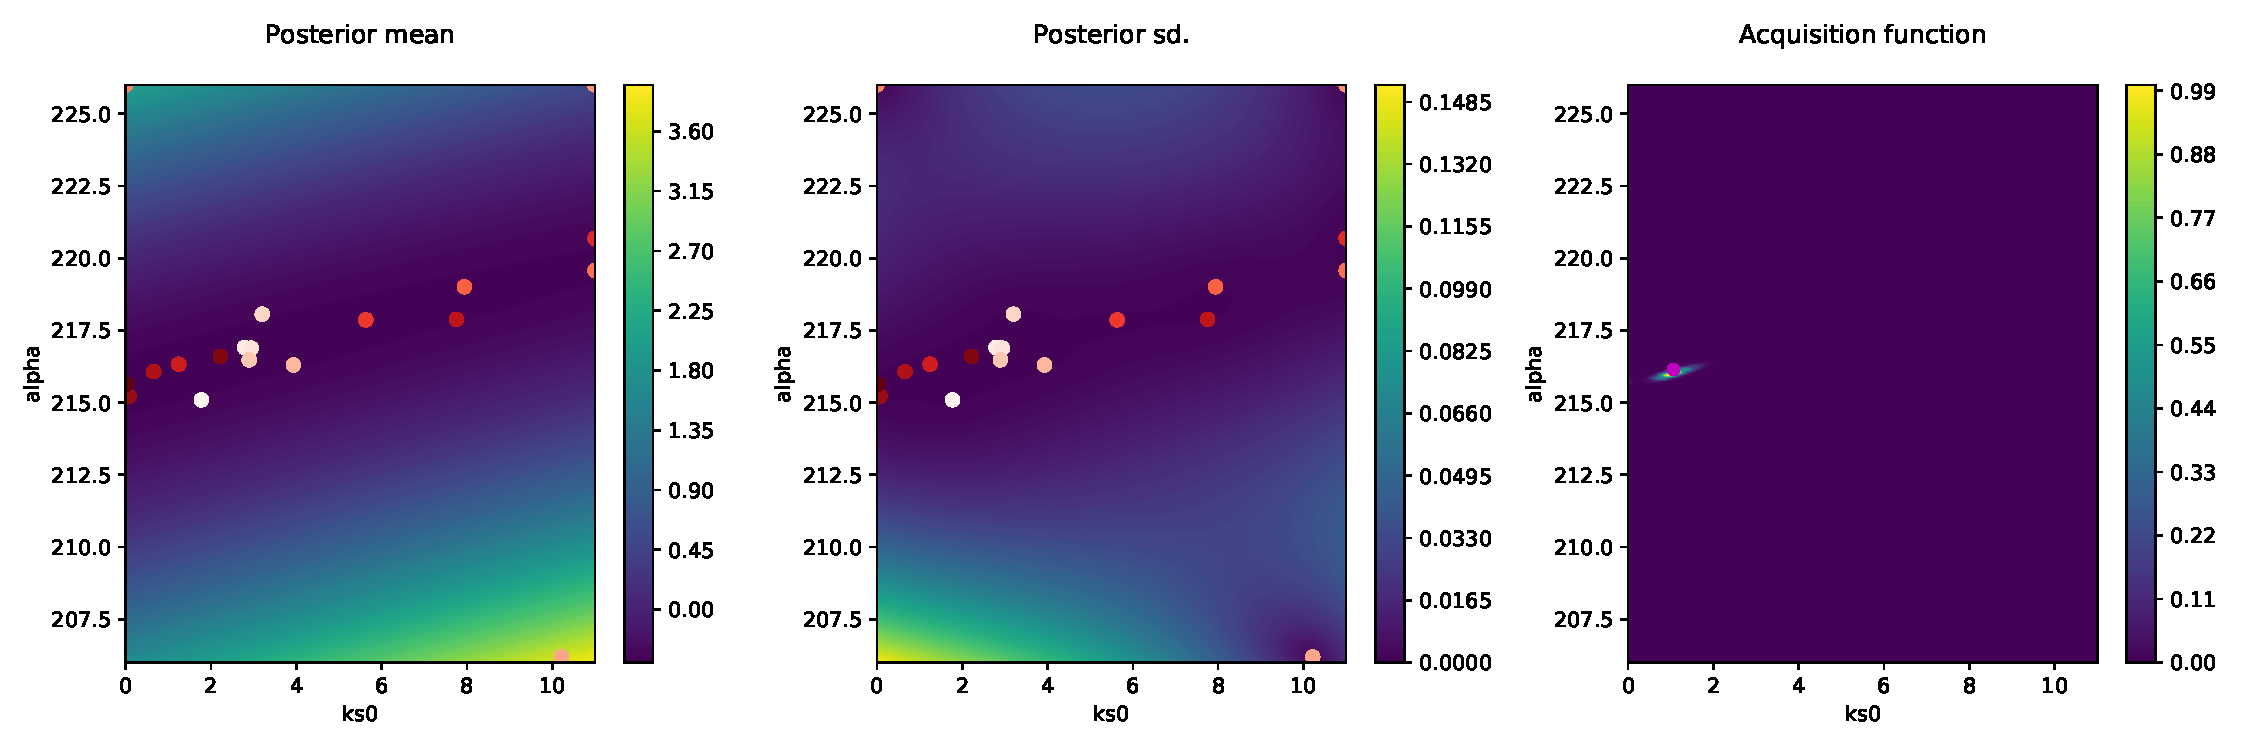
\includegraphics[width=0.7\textwidth]{Images/Multiple variables/2var_convergence_iter_20.pdf}
    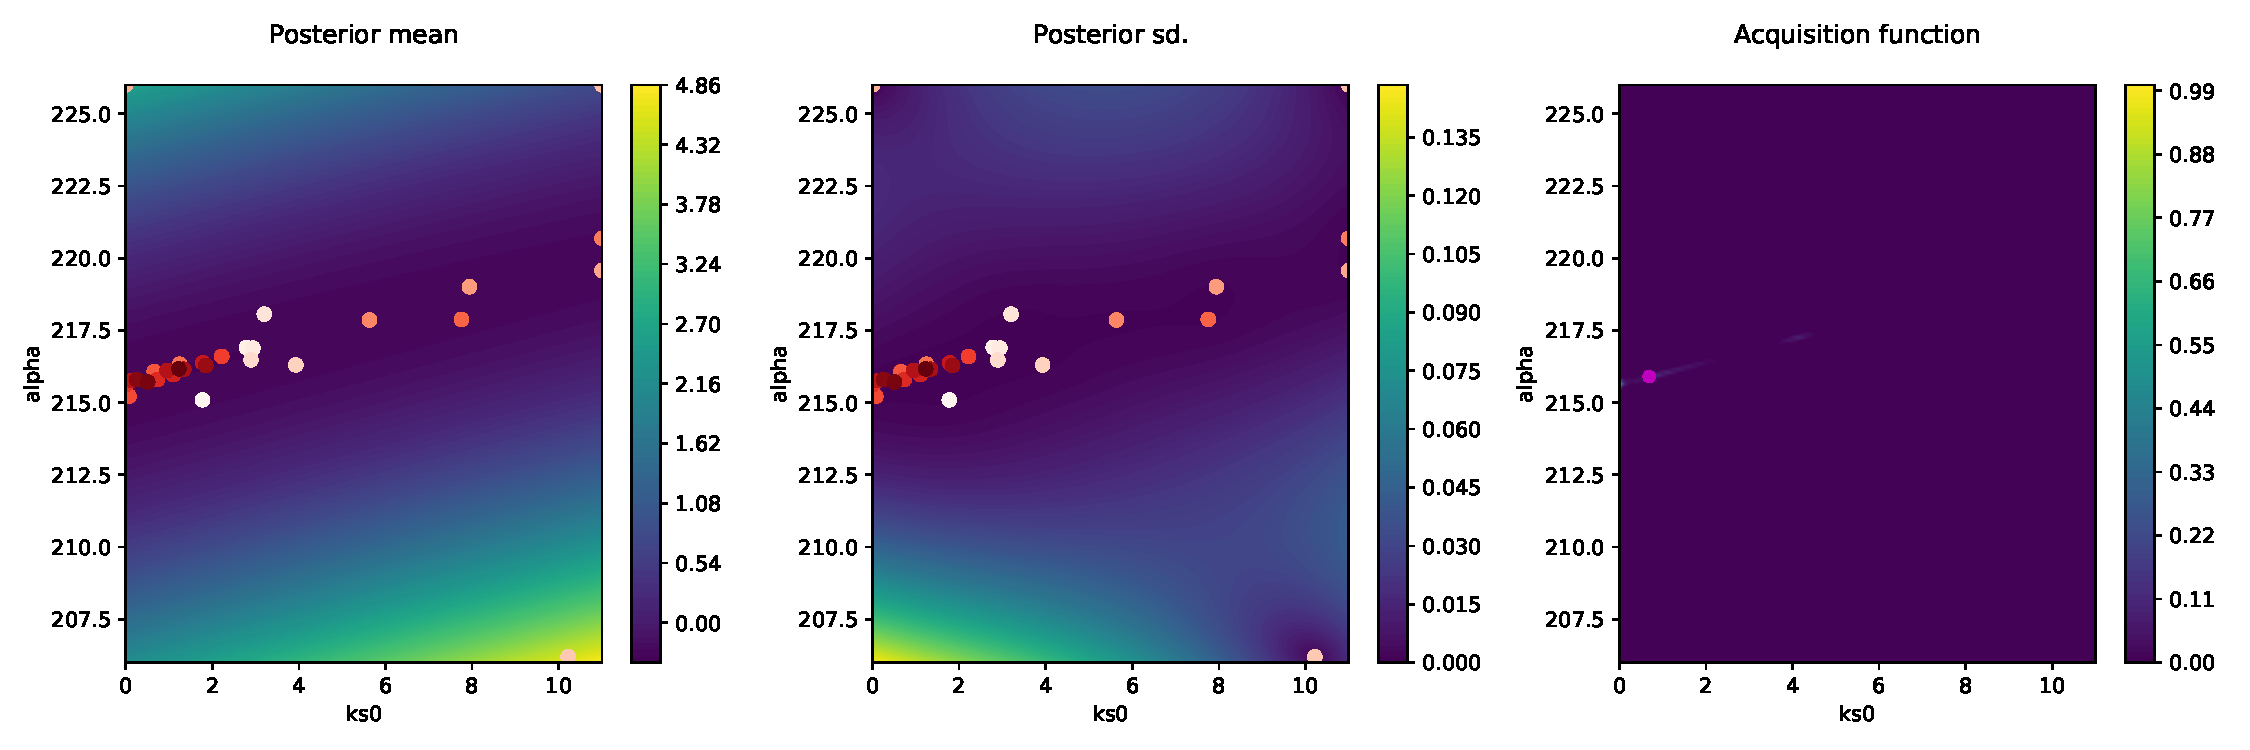
\includegraphics[width=0.7\textwidth]{Images/Multiple variables/2var_convergence_iter_30.pdf}
    \caption{Surrogate and acquisition function for BayesOpt inference of two parameters, $k_{s0}$ and $\alpha$ (nominal values 1.0 and 216.0, respectively), for successive iterations. The surrogate's mean and standard deviation are plotted separately. Iteration number from top to bottom: 1, 10, 20, 30.}
    \label{fig:2var_progression}
\end{figure}

For three-parameter inference, the algorithm would not converge. Therefore, I ran it for a fixed number of iterations (500) and inspected frequency counts similarly to the noisy setting (Section \ref{sec:results_noise}). While BayesOpt is relatively confident about the viable region for $k_{s0}$, its estimates for $\alpha$ and $\kappa$ are far from their nominal values (Fig. \ref{fig:3var_histogram}). In the case of $\alpha$, there is a concentration of samples around 222.5, whereas the samples for $\kappa$ are spread out and cover more or less uniformly the entire sampling space, except for a burst of samples around 10.0.

\begin{figure}[ht]
    \centering
    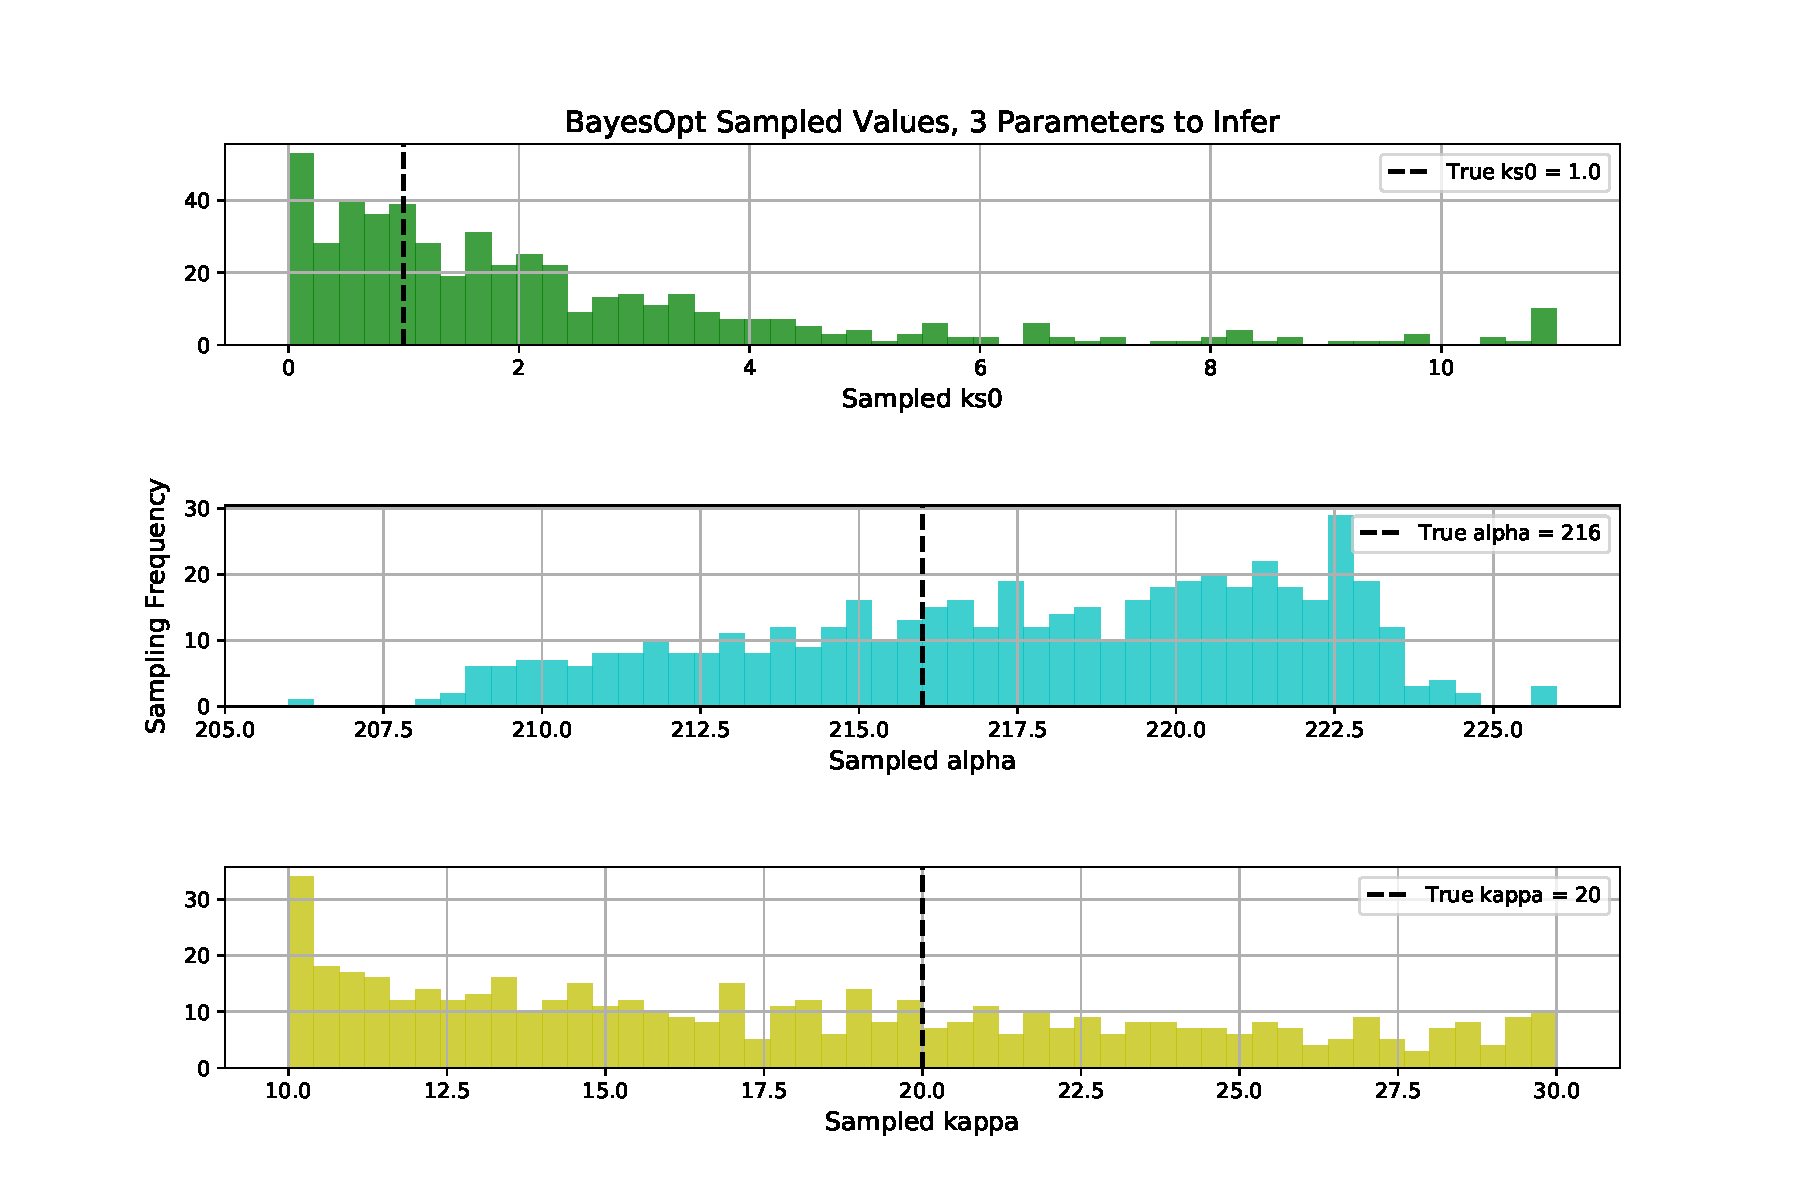
\includegraphics[width=0.8\textwidth]{Images/Multiple variables/Histogram_3var.pdf}
    \caption{Sampling frequency of BayesOpt-proposed values for 3-variable parameter inference ($k_{s0} = 1.0$, $\alpha=216.0$, $\kappa=20.0$). The algorithm has been run for a fixed number (500) of iterations.}
    \label{fig:3var_histogram}
\end{figure}

Similar results can be seen for the inference of four parameters (Fig. \ref{fig:4var_histogram}, note that here BayesOpt has been run for 1,000 iterations given the greater search space and curse of dimensionality problem discusses in Section \ref{sec:multiple}). In this case, it is the $nExp$ variable BayesOpt is confident about, while other values are sampled uniformly across the entire search space. This suggests the $nExp$ might be a 'stiff' parameter, while others might be 'sloppier' (extending over extended ranges with limited impact on overall objective landscape). An interesting feature to glean from the histograms is the presence of high sampling at the extremes of the search spaces for $k_{s)}$, $\alpha$ and $\kappa$. An explanation for this could be that BayesOpt fixes all parameter values but one, and explores the objective by varying only one parameter. This would also explain the spread of the samples between the two extremes.

The current experimental setting could be augmented in multiple ways:

\begin{enumerate}
    \item Run BayesOpt for a greater number of iterations. For the three- and four-parameter experiments, the iterations (500 and 1,000 respectively) could simply not be enough for the algorithm to converge. The computer used to perform the experiments posed serious limitations to their extent, and I had to balance a trade-off between breadth and depth for each one of them;
    
    \item The sampled solutions would need to undergo \textit{a posteriori} identifiability analysis, i.e. testing whether they are statistically significant by inspecting the objective landscape in the neighbourhood of the proposed vector parameters, as shown, for instance, in \cite{pmid18817540}.
\end{enumerate}

\begin{figure}[H]
    \centering
    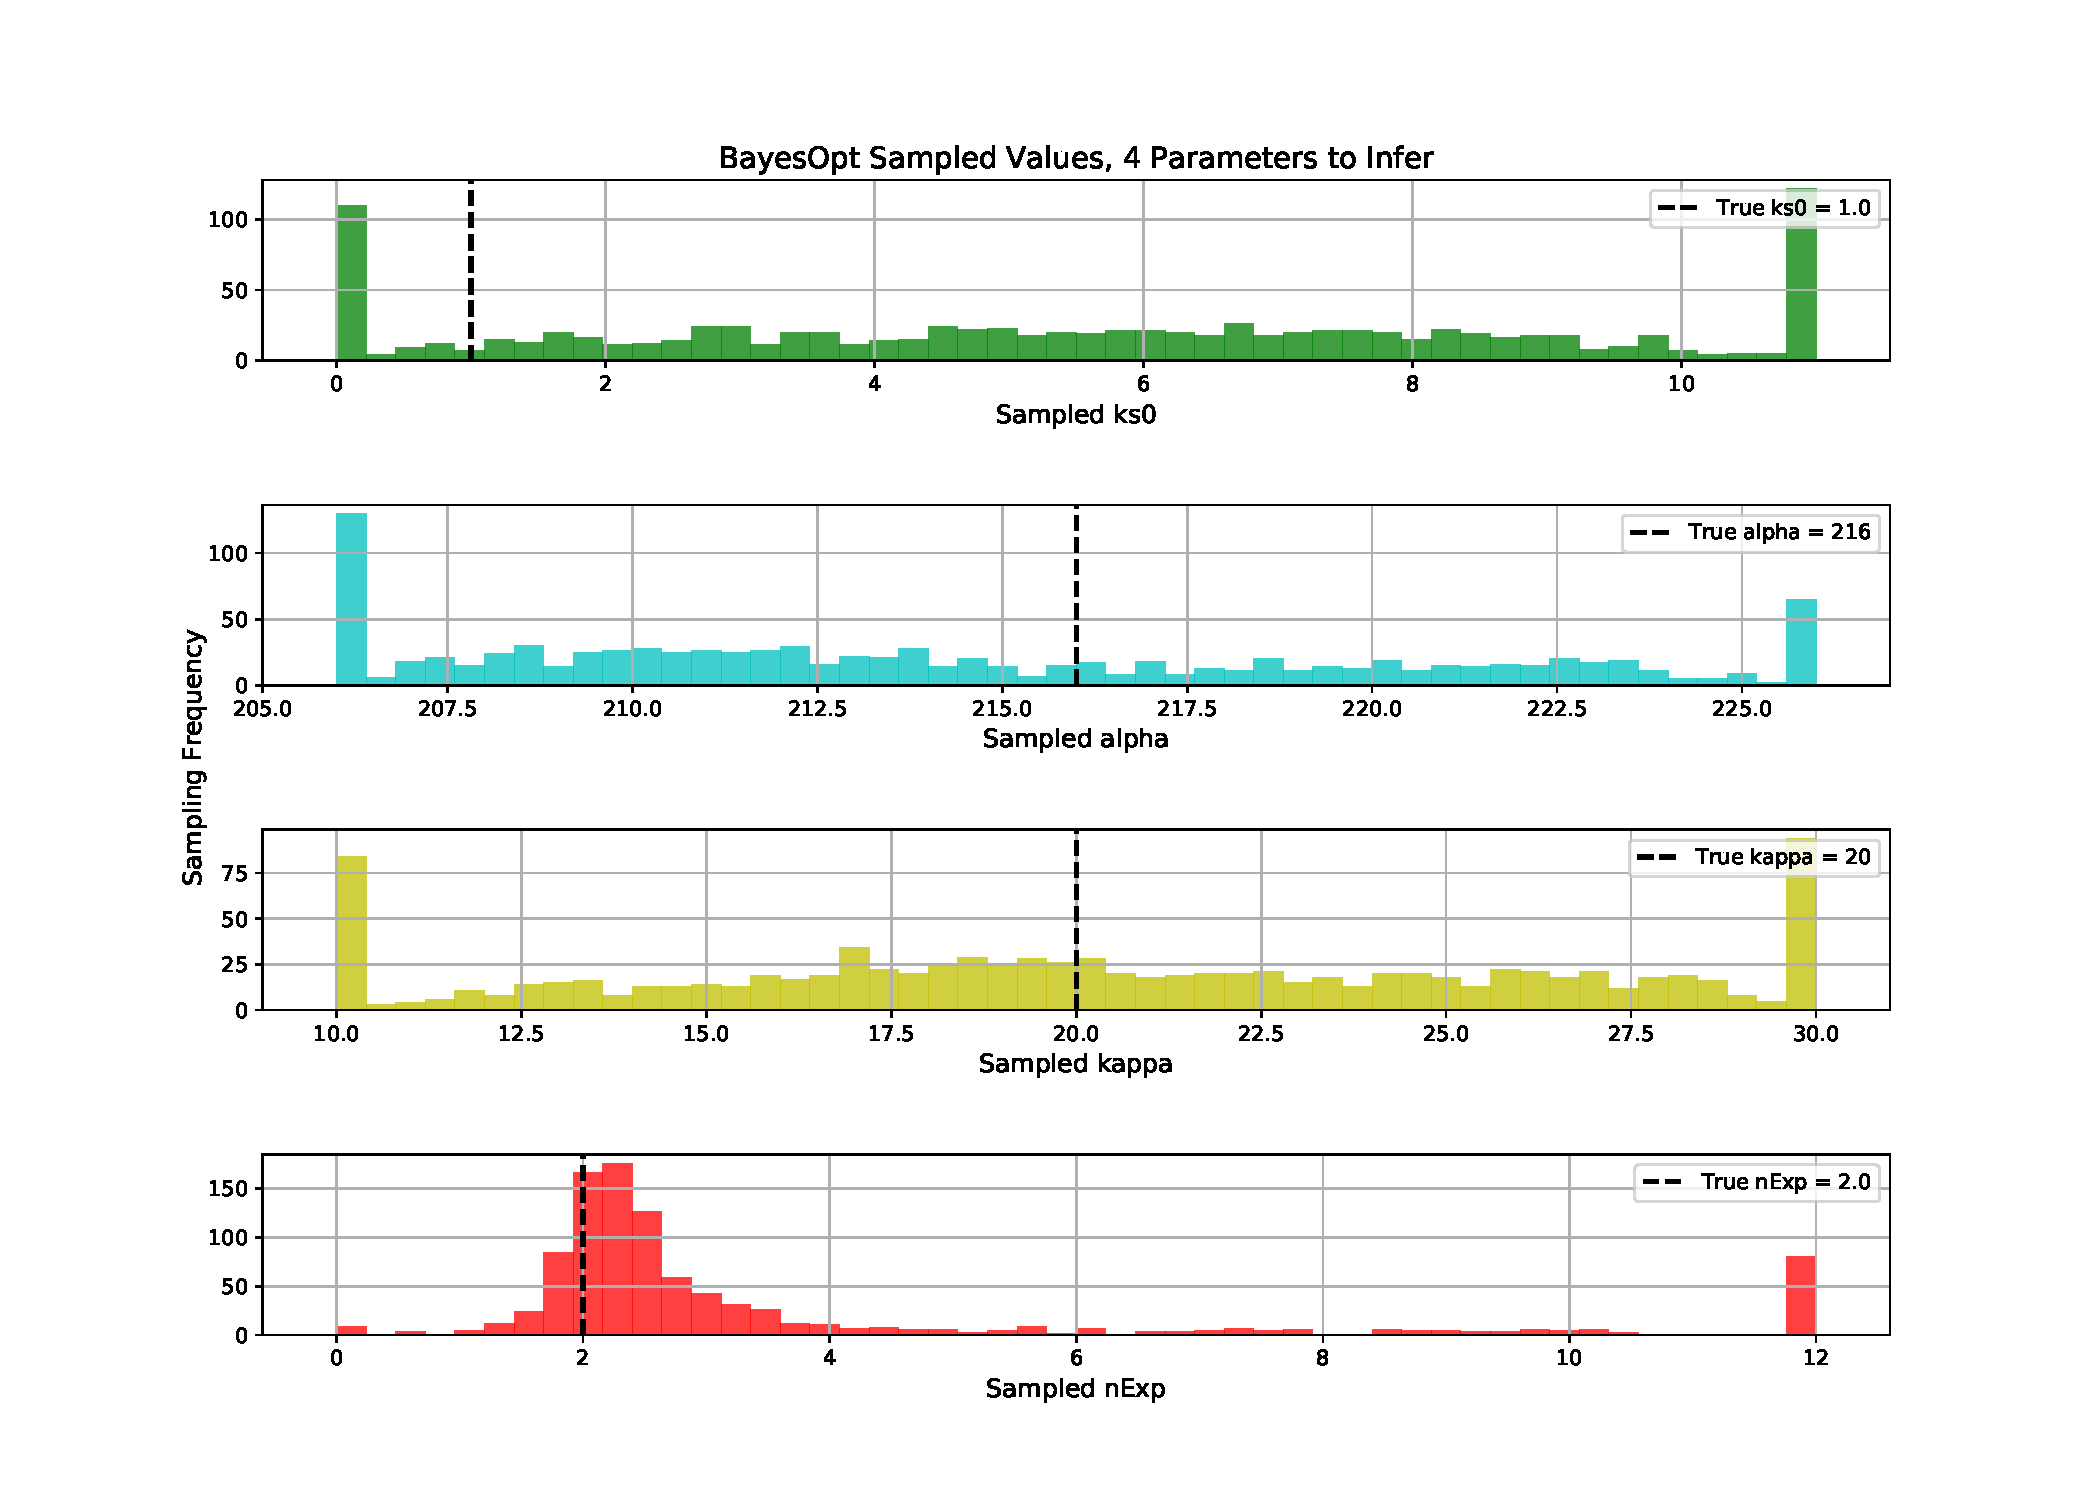
\includegraphics[width=0.8\textwidth]{Images/Multiple variables/Histogram_4var.pdf}
    \caption{Sampling frequency of BayesOpt-proposed values for 4-variable parameter inference ($k_{s0} = 1.0$, $\alpha=216.0$, $\kappa=20.0$, $nExp = 2.0$). The algorithm has been run for a fixed number (1,000) of iterations.}
    \label{fig:4var_histogram}
\end{figure}

\chapter{Conclusion}\label{ch:conclusion}
\section{Summary}
This thesis has explored the efficacy of Bayesian Optimization in the field of Systems Biology to infer parameters in multi-cellular simulations.

Chapter \ref{ch:background} provided a brief overview of the fields of Systems, Computational and Synthetic biology. It highlighted how a system-level understanding yields novel insights compared to a reductionist approach. It then delved into the computational and mathematical details of \textit{in silico} modelling, describing agent-based simulations and ordinary differential equations. Finally, it highlighted the importance of efficient parameter estimation techniques by comparing Markov Chain Monte Carlo and Bayesian Optimization.

Chapter \ref{ch:experiments} described different software packages for agent-based simulations, identifying Bsim as the optimal choice, as well as the libraries used for BayesOpt and MCMC. It also outlined the structure of the pipeline adopted throughout the experiments, and the conditions under which BayesOpt has been tested.

Finally, Chapter \ref{ch:conclusion} presented the results of the experiments. Bayesian Optimization has been shown to successfully estimate the correct parameter values under certain conditions. With variable-size search spaces, BayesOpt can correctly estimate parameters with a sampling range spanning up to four orders of magnitude. Noisy function evaluations make inference more difficult, and although an alternative acquisition function (Noisy Expected Improvement) has been implemented to deal with the issue, results show that a SNR $\approx$ 30-35dB still poses problems. Finally, simultaneous inference of two parameters terminates successfully in reasonable time, while for three- and four-parameter estimation results are inconclusive.

\section{Future Work}
Interesting directions for future research on the topic can extend this thesis in multiple ways:

\begin{itemize}
    \item Provided more computational resources, run BayesOpt for a greater number of iterations. I had to carefully balance breadth and depth of this work given time and computational constraints. A more complete analysis would inspect the behaviour of the algorithm over longer runs;
    
    \item Adopt different libraries. I have adopted GPyOpt as the library of choice due to its ease of implementation and relatively complete suite of functions. More complex alternatives such as BoTorch \cite{BoTorch}, optimized for GPU and parallel computing, could be used to conduct more intensive experiments:
    
    \item Test the implementation of MCMC provided in the supplemental material of this thesis. For time reasons, this was not thoroughly tested and therefore its results excluded from the final analysis. As the primary objective of this thesis was to compare BayesOpt against other frameworks, a natural continuation of this work would be to terminate implementation of MCMC and compare its accuracy and running time against BayesOpt's.  
\end{itemize}

\bibliographystyle{ieeetr}
\bibliography{mybibfile}

%% You can include appendices like this:
% \chapter*{Appendices}

% Manually add appendices to TOC since chapter*{} would not include it
% \addcontentsline{toc}{chapter}{Appendices}
% \appendix

% \chapter{Appendix Title}

% \section{First section}

% \subsection{First Subsection}

% \chapter{Appendix Title}
%
% Markers do not have to consider appendices. Make sure that your contributions
% are made clear in the main body of the dissertation (within the page limit).

\end{document}
